\documentclass{article}
\usepackage{polski}
\usepackage[utf8]{inputenc}
\usepackage{amsmath}
\usepackage{amsfonts}
\usepackage{mathtools}
\usepackage{graphicx}
\usepackage{subcaption}
\usepackage{float}
\usepackage{placeins}
\usepackage[left=2cm,right=2cm,top=2cm,bottom=2cm]{geometry}

\makeatletter
\newcommand{\mathleft}{\@fleqntrue\@mathmargin0pt}
\newcommand{\mathcenter}{\@fleqnfalse}
\makeatother


\graphicspath{{Obrazy/}}

\title{Teoria sterowania (TST)\\ PROJEKT 1}
\author{Arkadiusz Piórkowski}

\begin{document}
%\pagenumbering{gobble}
\maketitle

\section*{Zadanie}

\subsubsection*{Cel projektu}
Celem zadania jest zbadanie i zilustrowanie dynamiki układu liniowego
\[
x(t+1) = \bold{A}x(t), x(0)=x_0
\]
\[
\bold{A=\begin{bmatrix*}[r]
  a_{11} & a_{12} \\
  a_{21} & a_{22}
 \end{bmatrix*}}
\]
w przestrzeni fazowej.
\subsubsection*{Wymagania}
Badania i symulacje należy wykonać w rodowisku Matlab lub Octave, wykorzystując dostępne procedury numeryczne i graficzne. Stworzony skrypt powinien umożliwiać:
\begin{itemize}
\item konstruowanie macierzy o zadanym widmie,
\item konstruowanie zbioru \textbf{\textit{Z}} punktów początkowych rozłożonych na okręgu,
\item obliczanie trajektorii w przestrzeni stanów (portret fazowy),
\item obliczanie wektorów własnych $\nu_i$ macierzy \textbf{\textit{A}},
\item ilustrację obrazu \textbf{\textit{AZ}} zbioru \textbf{\textit{Z}} punktów położonych na okręgu jednostkowym,
\item ilustrację wektorów $\lambda_i\nu_i , \lambda_i \in \sigma(\bold {A}) , i =1,2$ ,
\item ilustrację pola wektorowego okr\'slającego trajektorie układu.
\end{itemize}
\subsubsection*{Zadania badawcze}
Należy wykonać następujące zadania:
\begin{itemize}
\item podać interpretację wartoci własnych i wektorów własnych,
\item zademonstrować zależno\'sć dynamiki układu od widma $\sigma(\bold{A}) = \{ \lambda \in \mathbb{C} : \varphi_A(\lambda) = 0 \}$ i wektorów własnych macierzy \textbf{\textit{A}}.
\end{itemize}

\section*{Sprawozdanie}
\subsection*{Wstęp teoretyczny}
Postać rozwiązania równania różnicowego liniowego:
\[
x(t+1) = \bold{A}x(t), x(0)=x_0
\]
jest następująca:
\[
x(t) = \bold{A}^t x_0
\]
Zatem dynamika układu jest okre\'slona przez własno\'sci ciągu $\bold{A}^t, t \to \infty$ . Własno\'sci tego ciągu są okre\'slone przez widmo macierzy \textbf{A} (zbiór pierwiastków równania charakterystycznego $\sigma(\bold{A}) = \{ z \in \mathbb{C} :\varphi_A(z) = 0 \}$). Z pierwiastkami równania charakterystycznego są związane wektory własne: $\lambda \in \sigma(\bold{A}) \Rightarrow \bold{A}x=\lambda x \wedge x\neq 0$.

W celu łatwiejszej analizy można skorzystać z podobieństwa macierzy $\bold{A}~i~\bold{J}$, które spełniają następujące równania:
\[
\bold{A} = \bold{PJP^{-1}} \equiv \bold{J} = \bold{P^{-1}AP}
\]
Podobieństwo nie zmienia widma
\[
\bold{A}x=\lambda x \Rightarrow \bold{J(P^{-1}}x) = \lambda(\bold{P^{-1}}x)
\]
\[
\sigma(\bold{A}) = \sigma(\bold{J})
\]
, ale transformuje wektory własne odwracalną macierzą zmiany bazy: $z = \bold{P^{-1}}x$.
\newline \newline
Dynamika długookresowa jest okre\'slona przez widmo $\sigma(\bold{A}) = \sigma(\bold{J})$, o czym \'swiadczy:
\begin{gather*}
\begin{aligned}
\bold{A} &= \bold{PJP^{-1}} \\
\bold{A^2} &= \bold{PJP^{-1}PJP^{-1}}=\bold{PJ^2P^{-1}}\\
&~\vdots\\
\bold{A^t} &= \bold{PJ^tP^{-1}}
\end{aligned}
\end{gather*}
Postać diagonalna macierzy ułatwia analizę dynamiki układu, ale nie każdą macierz można zdiagonalizować. Istnieje jednak postać macierzy bliskiej diagonalnej, która zachowuje widmo. Są to macierze Jordana, które są podobne do dowolnej macierzy kwadratowej. Macierze Jordana $\bold{J}$ posiada na diagonali klatki Jordana $\bold{J_i}$, które są związane z warto\'sciami własnymi $\lambda_i$ :
\begin{gather*}
\begin{aligned}
\bold{J} &= diag(\bold{J_1,\dots,J_m}), 1 \le m \le n \\
\bold{J_i} &= [b_{kl}]_{s_i \times s_i} = \lambda_i\bold{I} +\bold{N_i}, \sum_{i=1}^{m} s_i = n
\end{aligned}
\end{gather*}
, gdzie macierz $N_i$ jest macierzą nilpotentną posiadającą jedynki powyżej diagonali:
\[
\bold{N_i}=\begin{bmatrix*}[r]
  0 & 1 & \cdots & 0 & 0\\
  0 & 0 & \cdots & 0 & 0\\
  \vdots&\vdots&\ddots&\vdots&\vdots\\
  0 & 0 & \cdots & 0 & 1\\
  0 & 0 & \cdots & 0 & 0
 \end{bmatrix*}_{s_i \times s_i}
\]
\pagebreak

\section{Konstruowanie macierzy $\bold{A}$ o zadanym widmie i obliczanie wektorów własnych $\nu_i$ macierzy}

Do konstruowania macierzy o zadanym widmie posłużono się podobieństwem macierzy $\bold{A}$ i macierzy Jordana $\bold{J}$, o okre\'slonej strukurze
\[
\bold{A} = \bold{PJP^{-1}}
\]
, gdzie :
 \[
\bold{J}=\begin{bmatrix*}[r]
  \lambda_1 & 0\\
  0 & \lambda_2 
  \end{bmatrix*}
\]
Macierz zmiany bazy $\bold{P}$ musi być macierzą nieosobliwą. \newline
Zatem ciąg $\bold{A}^t, t \to \infty$ jest zależny od warto\'sci własnych:
\[
\bold{A} = \bold{P
\begin{bmatrix*}[r]
  \lambda_1^t & 0\\
  0 & \lambda_2^t 
  \end{bmatrix*}
  P^{-1}}
\]
Dodatkowo umożliwiono tworzenie macierzy o zespolonych sprzężonych warto\'sciach własnych:
 \[
\bold{A}=\begin{bmatrix*}[r]
  a & b\\
  -b & a 
  \end{bmatrix*}
\]
Widmo takiej macierzy ma następującą postać
\[
\sigma(\bold{A})=\{a \pm bi\}
\]
Poniżej przedtsawiono fragment kodu umożliwiający tworzenie macierzy o zadanym widmie:
\begin{verbatim}
%% Konstruowanie macierzy o zadanym widmie
clear variables;
J = [ 0.2 0; 0 0.2]; %widmo rzeczywiste
P = [ 3 13; 11 1];
A = P*J/P; %macierz o zadanym widmie sigma(J)
%A = [0.4 0.7; -0.7 0.4]; %A=[a b;-b,a] => widmo a+-ib;
\end{verbatim}
Obliczanie wektorów własnych wykonano za pomocą polecenia programu Matlab \textit{eig()} :
\begin{verbatim}
%% obliczanie wektorow wlasnych v_i macierzy A
%wartosci wlasne
[L] = eig(A);
%wektory wlasne(kolumnowo) i wartosci wlasne w postaci macierzy Jordana
[V, J] = eig(A);
\end{verbatim}
, gdzie: \newline
L - wektor warto\'sci własnych \newline
V - macierz wektorów własnych(kolumnowo) \newline
J - macierz diagonala z warot\'sciami własnymi.


\section{Konstruowanie zbioru Z punktów początkowych rozłożonych na okręgu}

Zbiór punktów początkowych jest rozłożony co $\frac{\pi}{4}$ od 0 do $2\pi$ na okręgu jednostkowym.
Fragment kodu:
\begin{verbatim}
%% Konstruowanie zbioru Z punktów poczatkowych rozlozonych na okregu
theta=0:pi/100:2*pi;
radius=1;
z=radius*exp(1i*theta);
Z=[real(z);imag(z)];

points=0:pi/4:2*pi;
x0=radius*exp(1i*points);
X0=[real(x0);imag(x0)];

fig1=figure(1);hold on; grid on;
plot(Z(1,:),Z(2,:),'b',X0(1,:),X0(2,:),'ko','MarkerFace','r');
axis equal;
hold on;
\end{verbatim}
\begin{figure}[H]
	\centering
	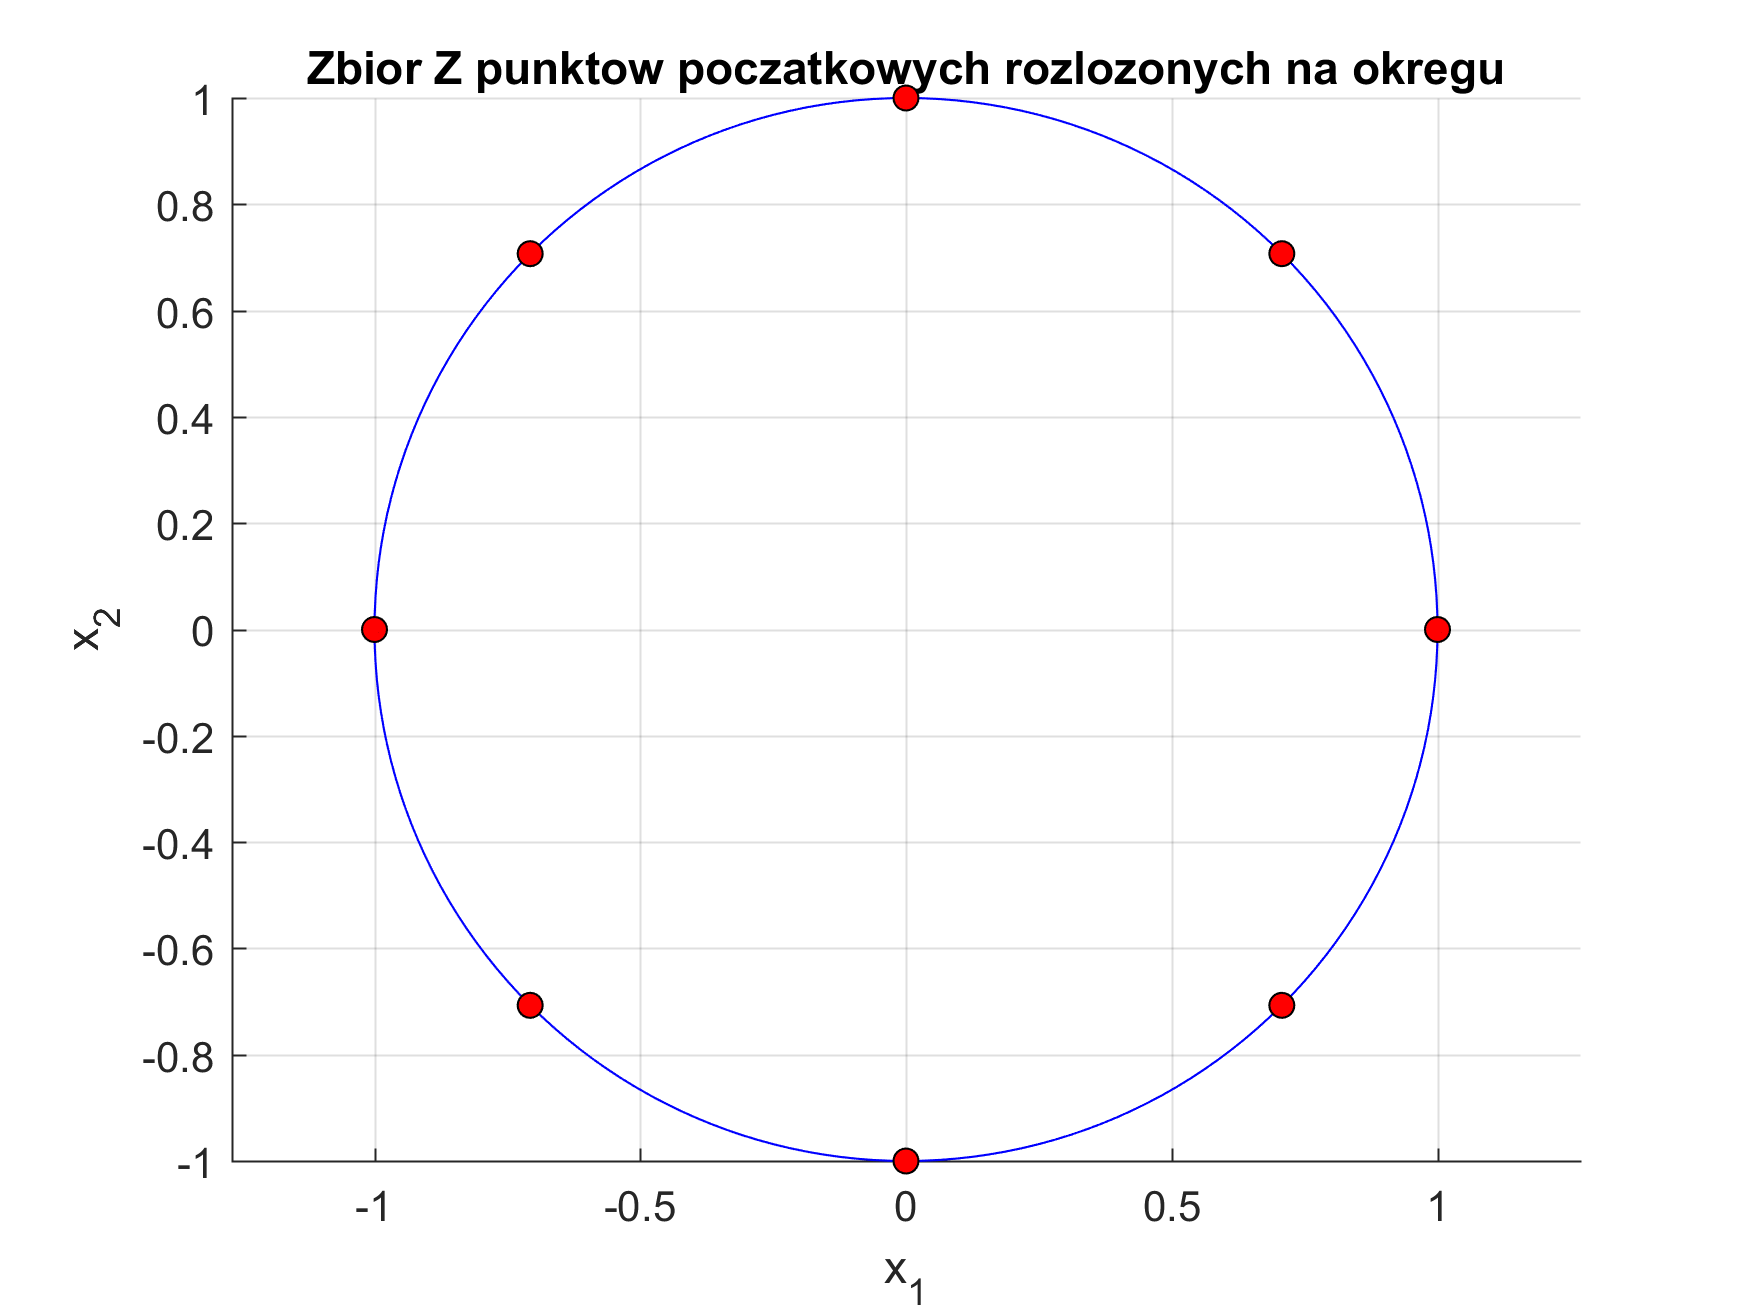
\includegraphics[width=0.8\textwidth]{zbior_punktow_poczatkowych.png}
	\caption{Zbiór punktów początkowychi}
	\label{fig::punkty_początkowe}
\end{figure}

\section{Obliczanie trajektorii układu (rozwiązań równania stanu) dla wybranych punktów początkowych i pola wektorowego}

Wyznaczenie trajektorii układu polegało na rozwiązniu równania różnicowego liniowego dla kolejnych chwil czasu~$t$:
\[
x(t+1) = \bold{A}x(t), x(0)=x_0
\]
, co sproawdza się do obliczenia kolejnych wyrazów ciągu:
\[
x(t) = \bold{A^t}x_0
\]
Fragment kodu realizujący podane zadanie:
\begin{verbatim}
%% obliczanie trajektorii ukladu (rozwiazan r-nia stanu) dla wybranych punktow poczatkowych

iter=40;
x1=zeros(iter,length(points));
x2=zeros(iter,length(points));

for i=1:length(points)
    for j=1:iter
        if j==1
            x1(j,i)=X0(1,i);
            x2(j,i)=X0(2,i);
        else
            x1(j,i)=A(1,1)*x1(j-1,i) + A(1,2)*x2(j-1,i);
            x2(j,i)=A(2,1)*x1(j-1,i) + A(2,2)*x2(j-1,i);
        end
    end
end
\end{verbatim}

Pole wektorowe okre\'slające trajektorie układu obliczono według wzoru:
\begin{gather*}
\begin{aligned}
x(t+1)&=\bold{A}x(t); \\
\Delta x(t) &= x(t+1) - x(t) = (\bold{A-I})x(t)
\end{aligned}
\end{gather*}

\section{Ilustracja otrzymanych wyników}

W danym punkcie przedstawiono ilustracje: 
\begin{itemize}
\item[-] trajektorii w przestrzeni stanów(portret fazowy),
\item[-] obrazu \textit{\textbf{AZ}} zbioru \textit{\textbf{Z}} punktów położonych na okręgu jednostkowym, 
\item[-] wektorów $\lambda_i\nu_i , \lambda_i \in \sigma(\bold {A}) , i =1,2$ ,
\item[-] pola wektorowego okr\'slającego trajektorie układu,
\end{itemize}
dla różnych warto\'sci własnych macierzy \textit{\textbf{A}} (widma $\sigma(\bold{A}) = \{ \lambda \in \mathbb{C} : \varphi_A(\lambda) = 0 \}$.

\begin{figure}[H]
    \centering
    \begin{subfigure}{0.44\textwidth}
        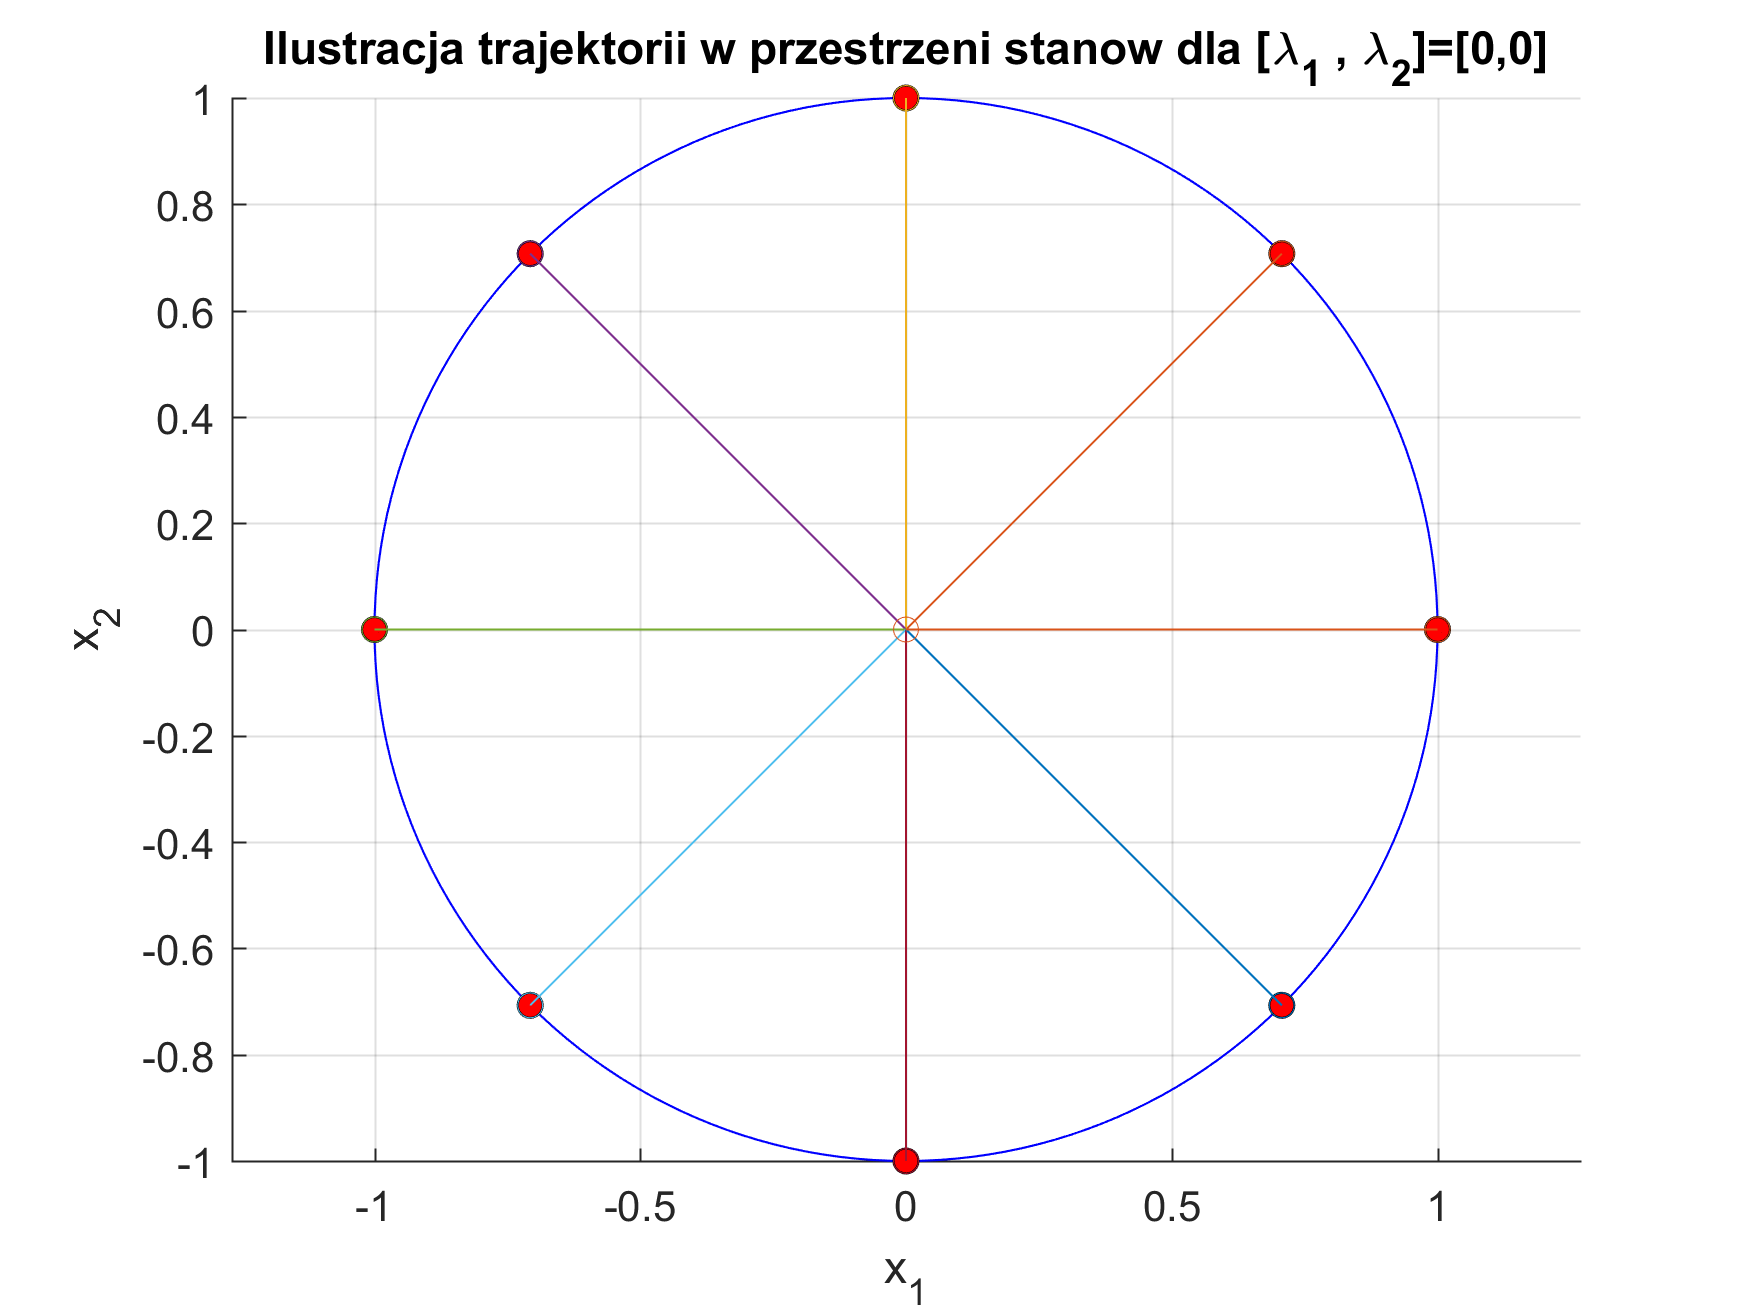
\includegraphics[width=\textwidth]{portret_fazowy_0_0.png}
    \end{subfigure}
    \begin{subfigure}{0.48\textwidth}
        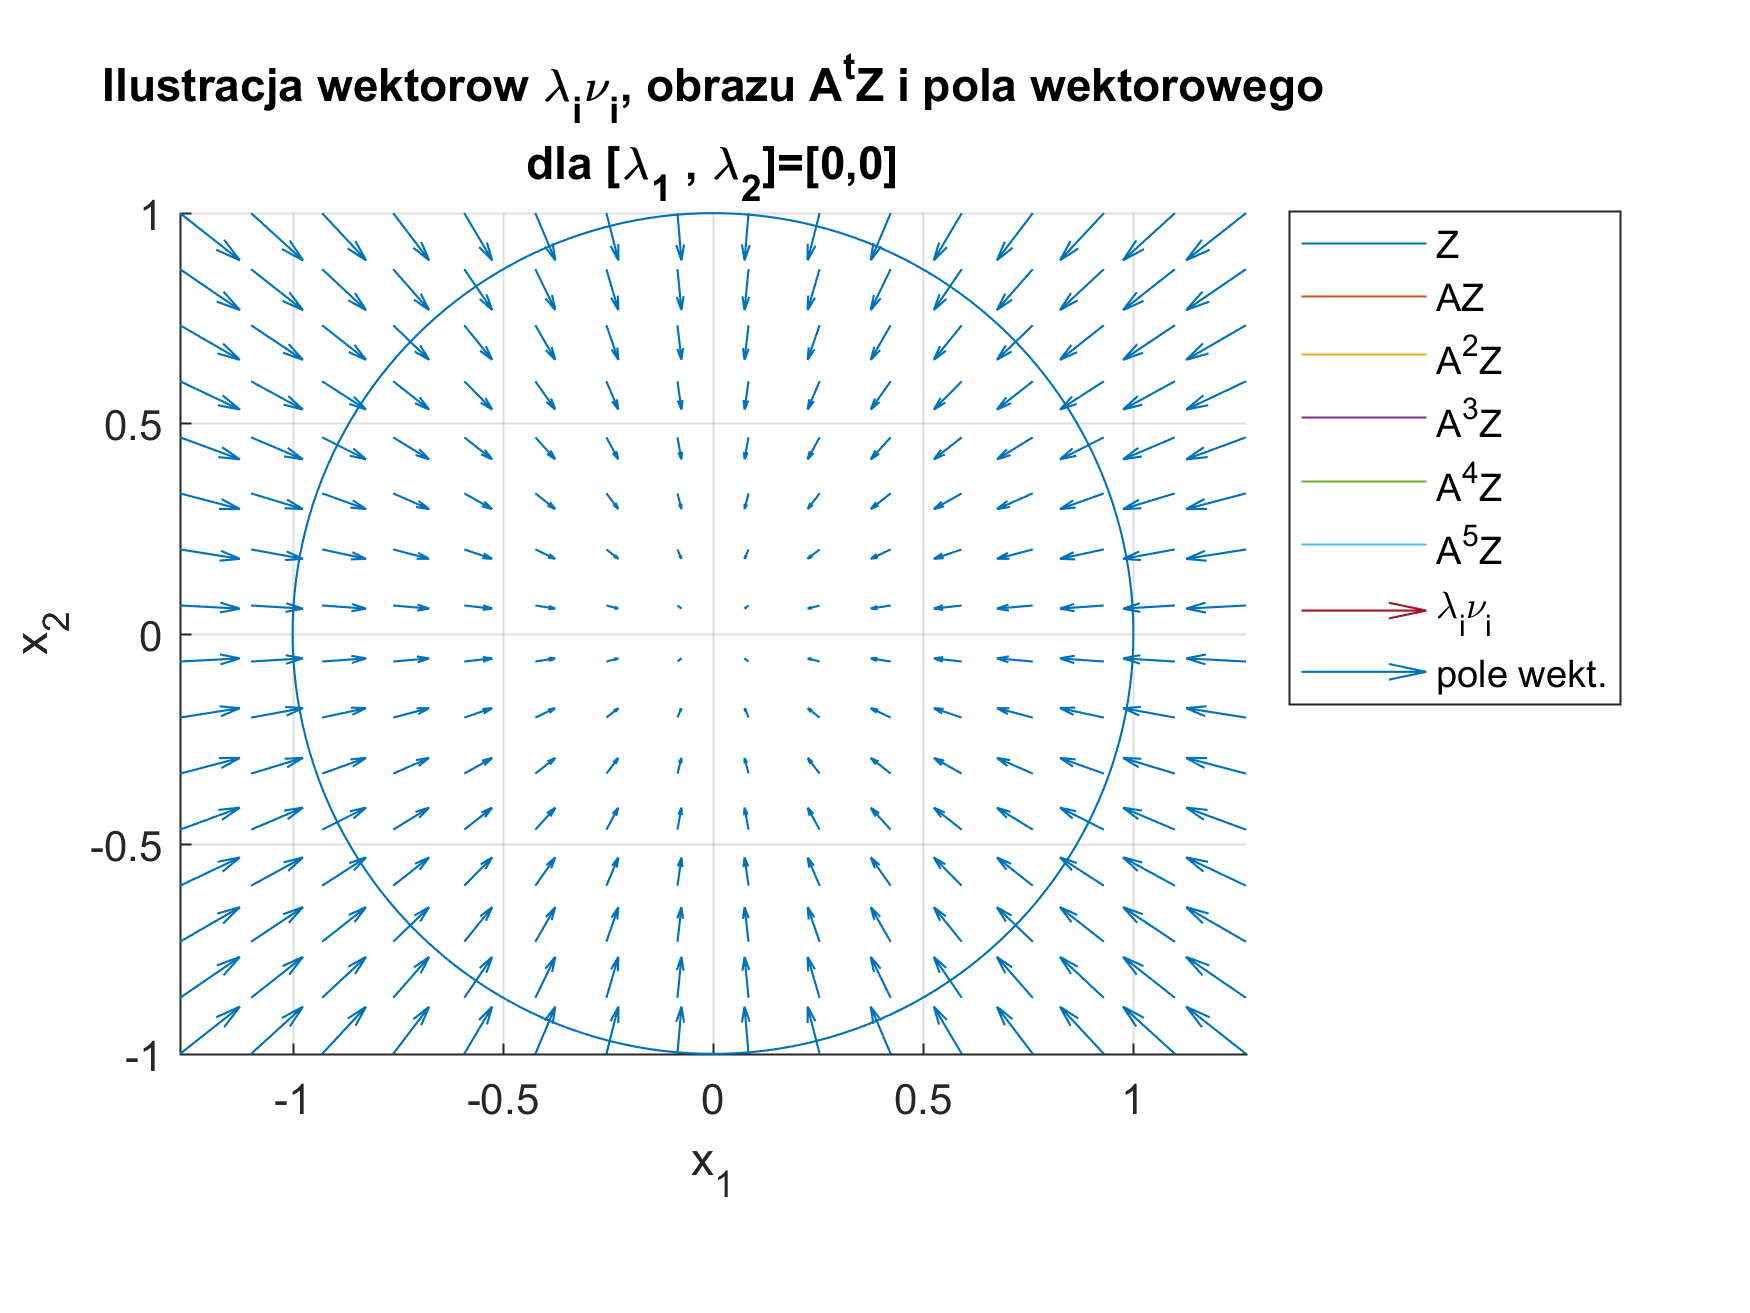
\includegraphics[width=\textwidth]{pole_wektorowe_0_0.png}
    \end{subfigure}
    \caption{Warto\'sci własne $[ \lambda_1, \lambda_2 ]= [ 0, 0 ]$}
    \label{fig::0i0}
\end{figure}
\begin{figure}[H]
    \centering
    \begin{subfigure}{0.44\textwidth}
        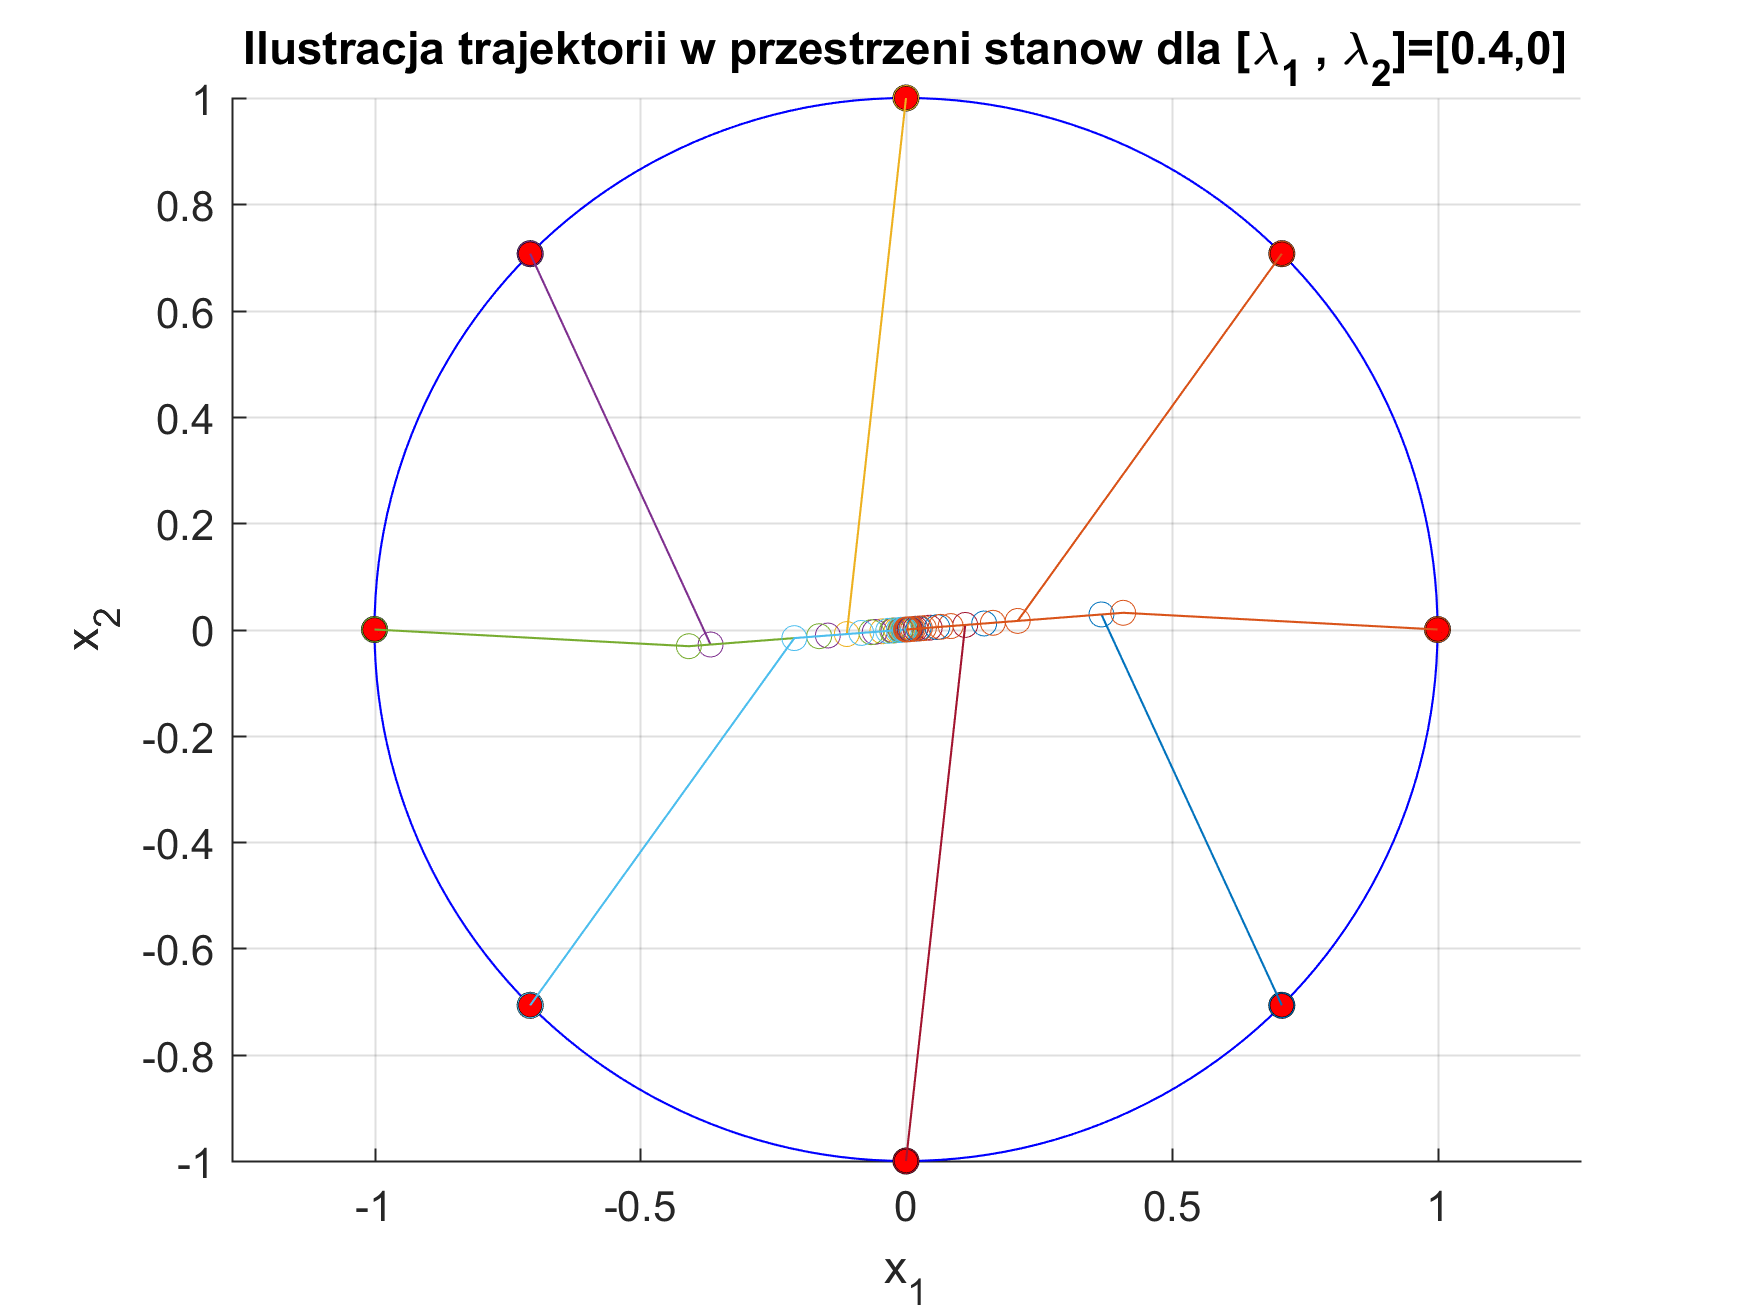
\includegraphics[width=\textwidth]{portret_fazowy_4_0.png}
    \end{subfigure}
    \begin{subfigure}{0.48\textwidth}
        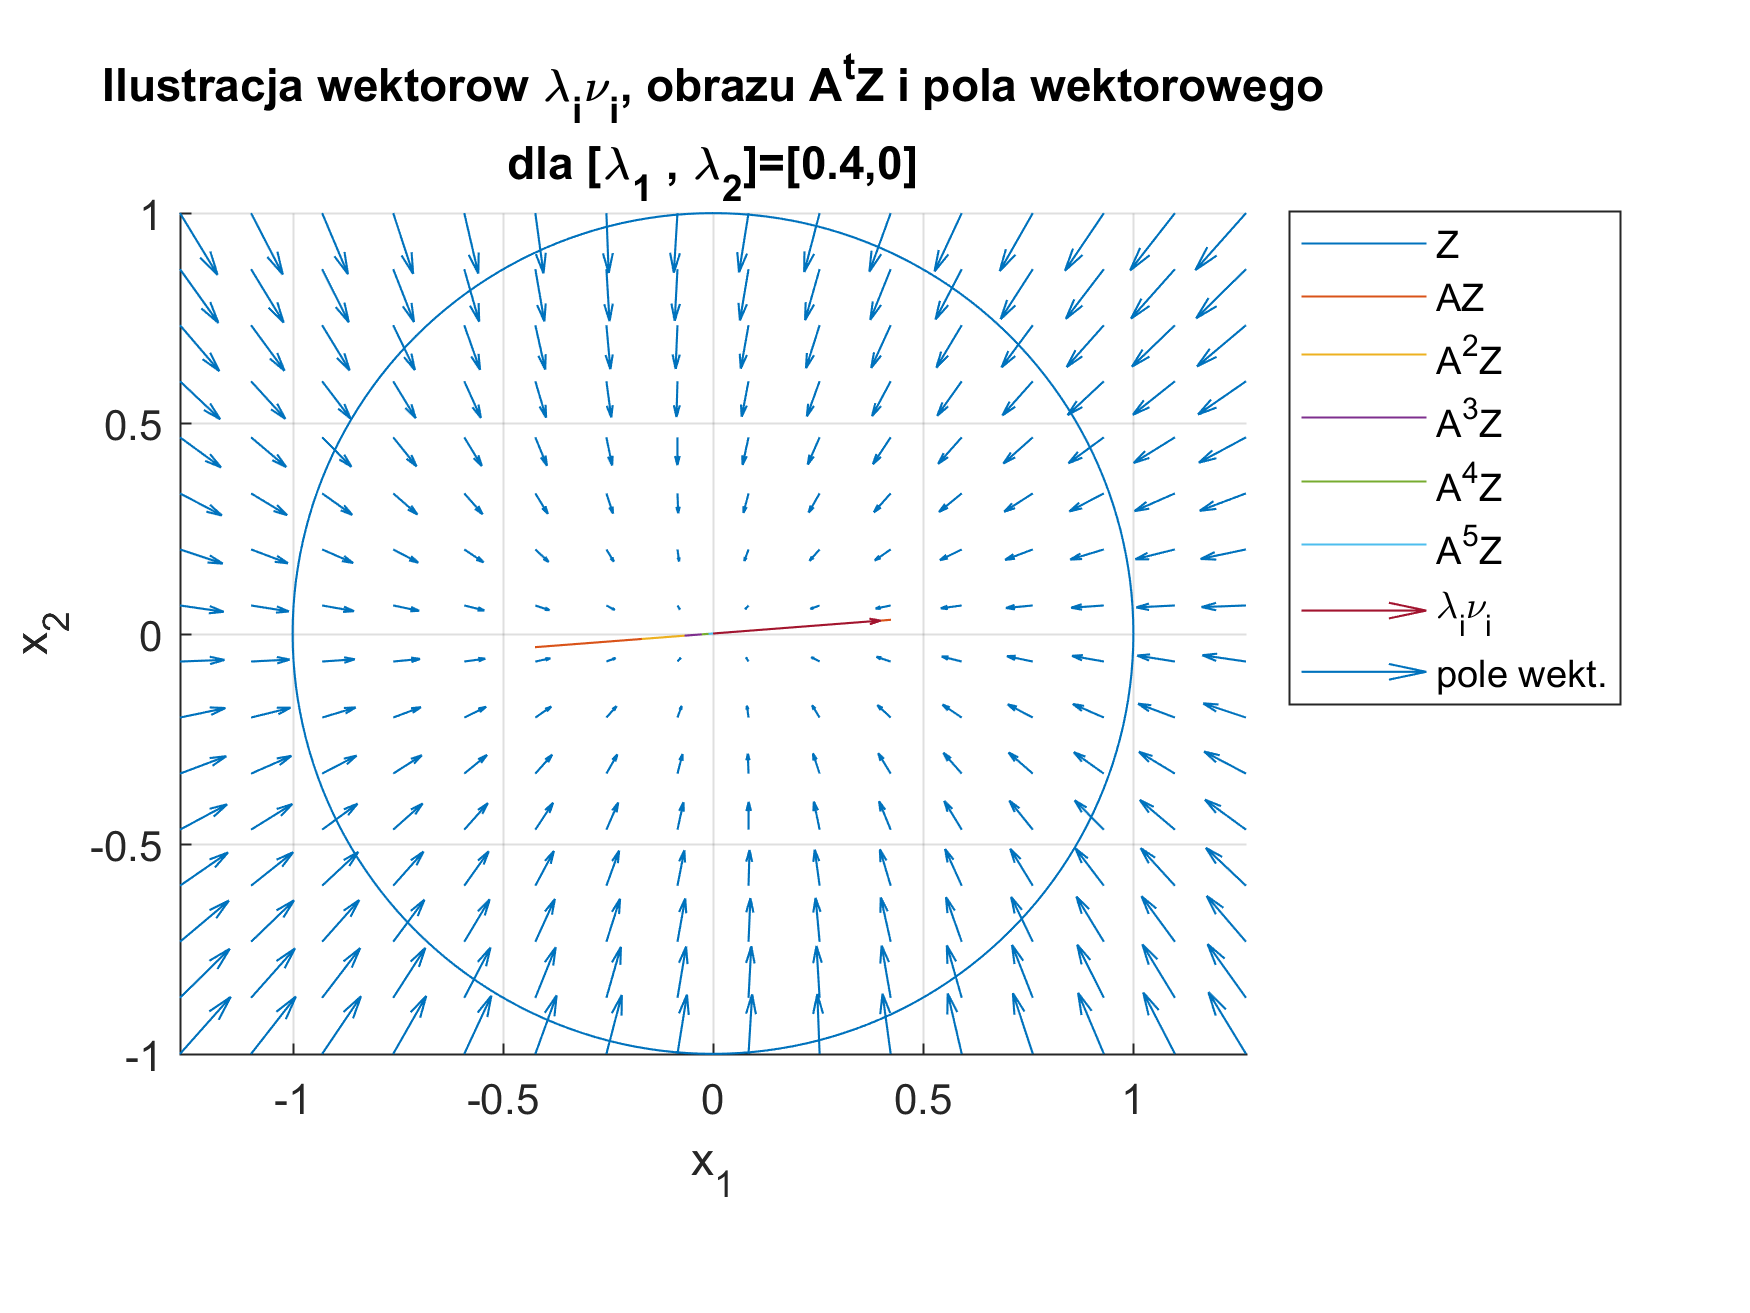
\includegraphics[width=\textwidth]{pole_wektorowe_4_0.png}
    \end{subfigure}
    \caption{Warto\'sci własne $[ \lambda_1, \lambda_2 ]= [ 0.4, 0 ]$}
    \label{fig::4i0}
\end{figure}
\begin{figure}[H]
    \centering
    \begin{subfigure}{0.44\textwidth}
        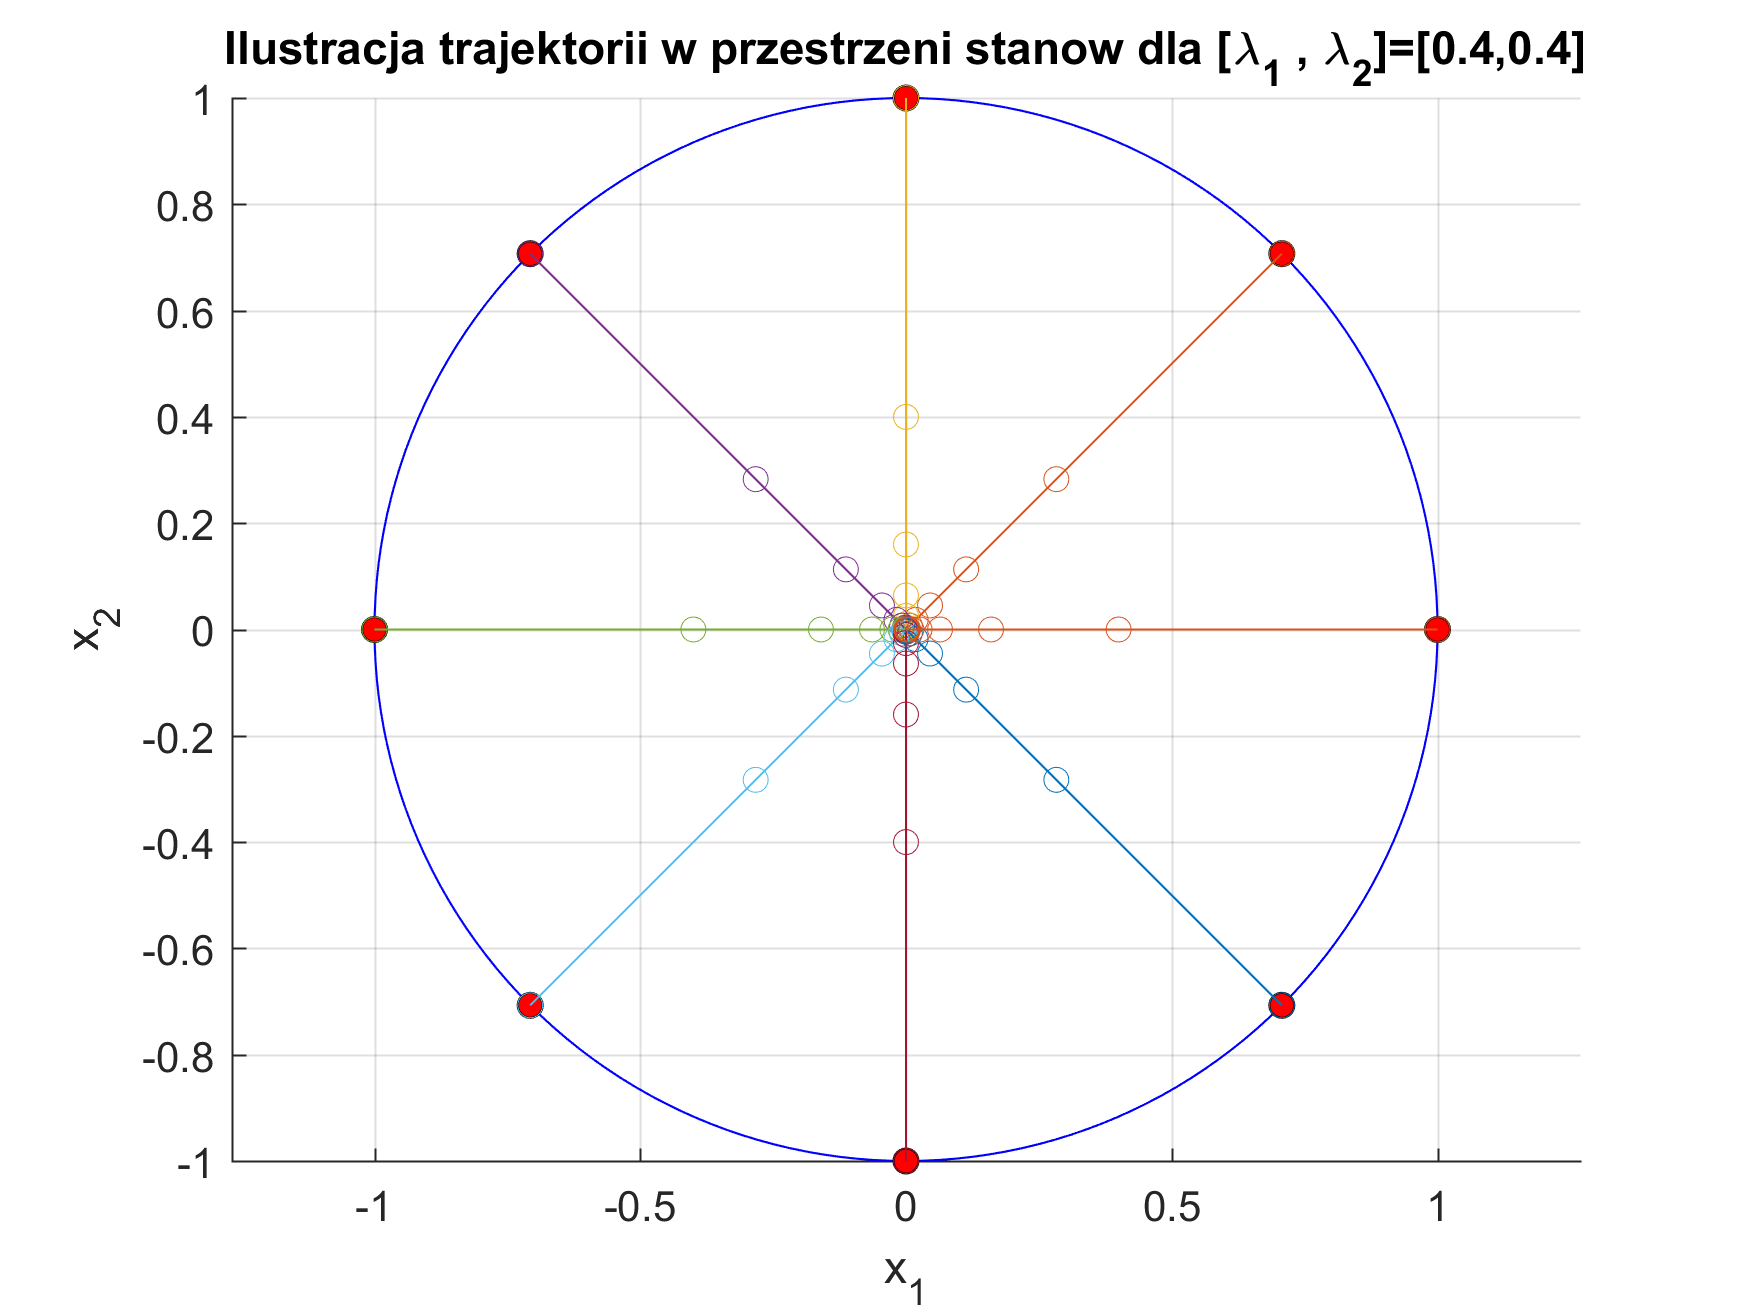
\includegraphics[width=\textwidth]{portret_fazowy_4_4.png}
    \end{subfigure}
    \begin{subfigure}{0.48\textwidth}
        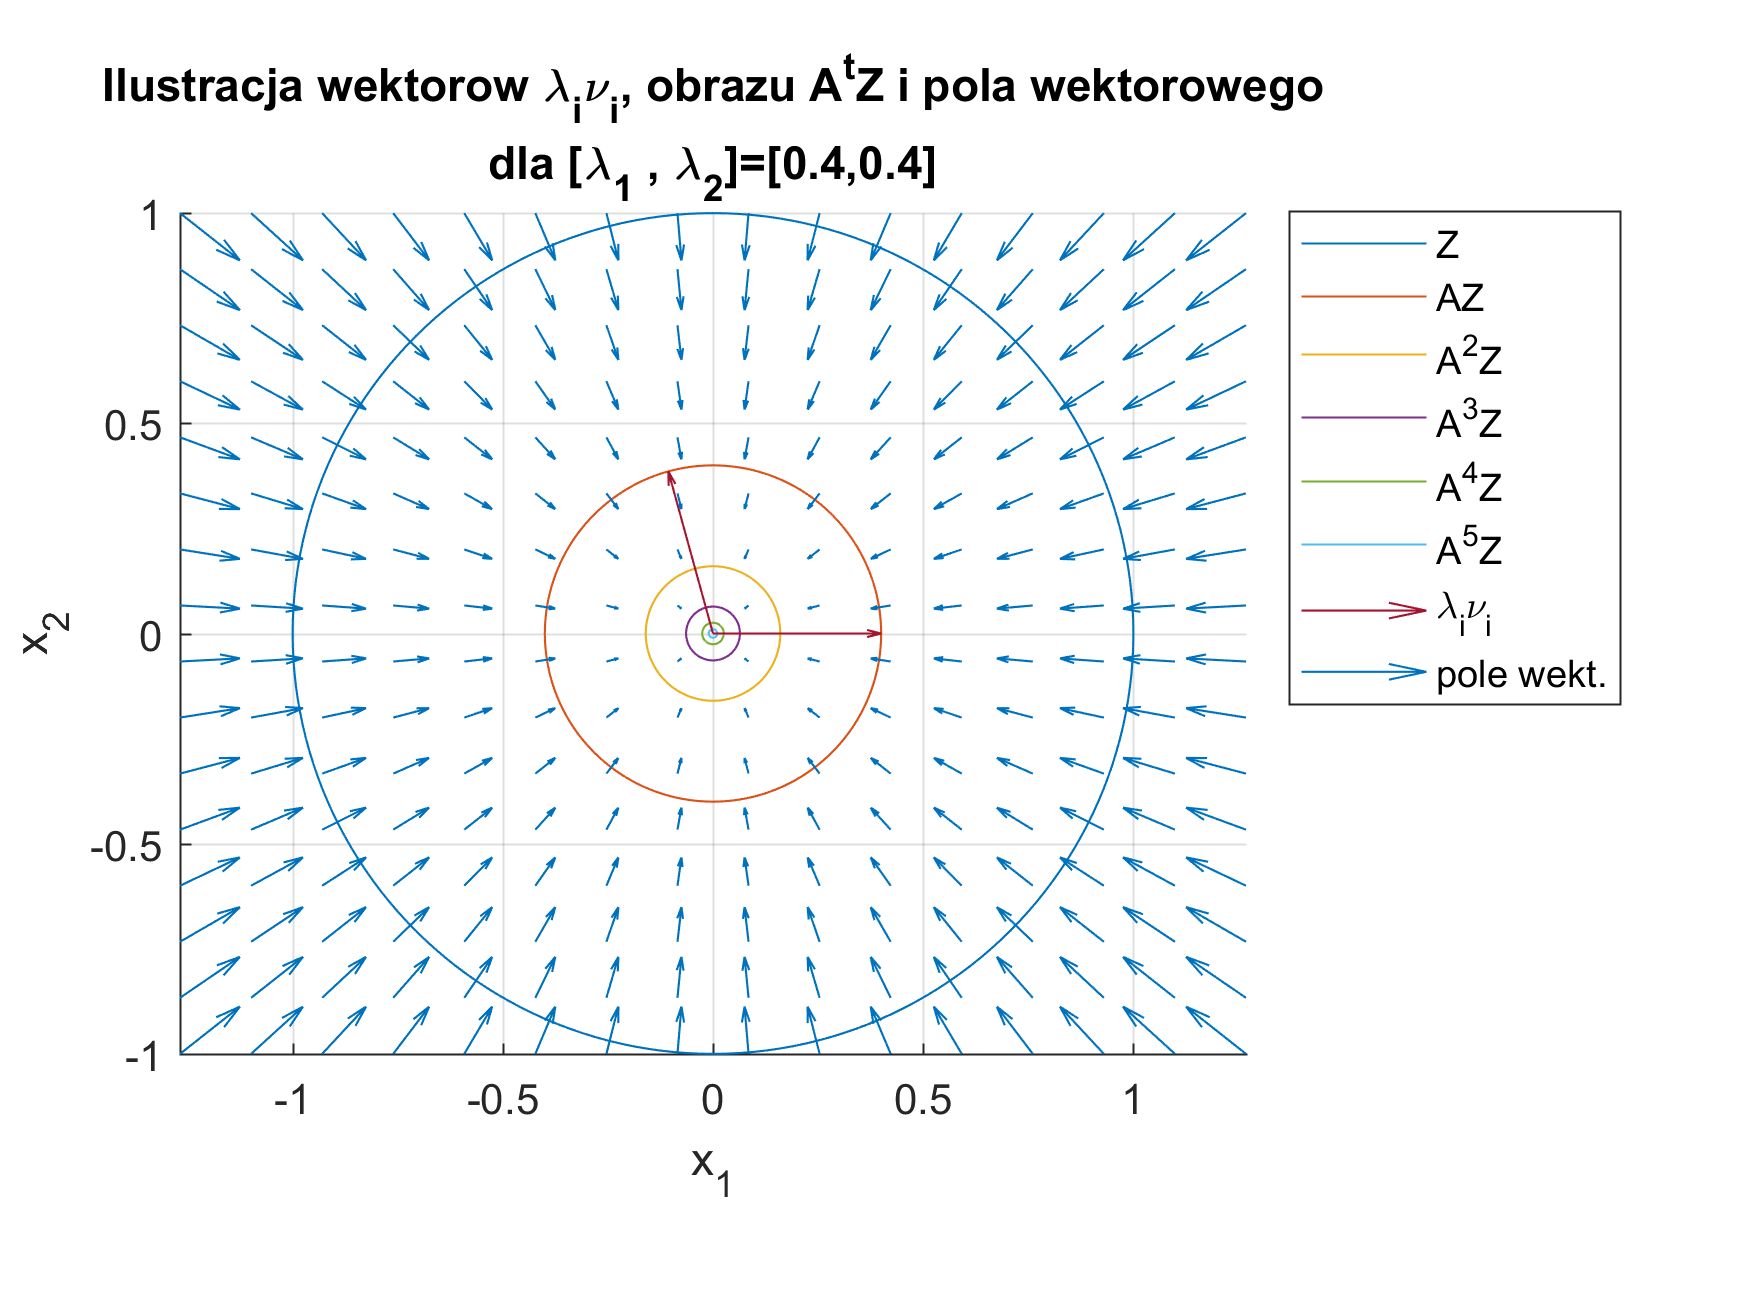
\includegraphics[width=\textwidth]{pole_wektorowe_4_4.png}
    \end{subfigure}
    \caption{Warto\'sci własne $[ \lambda_1, \lambda_2 ]= [ 0.4, 0.4 ]$}
    \label{fig::4i4}
\end{figure}

\begin{figure}[H]
    \centering
    \begin{subfigure}{0.44\textwidth}
        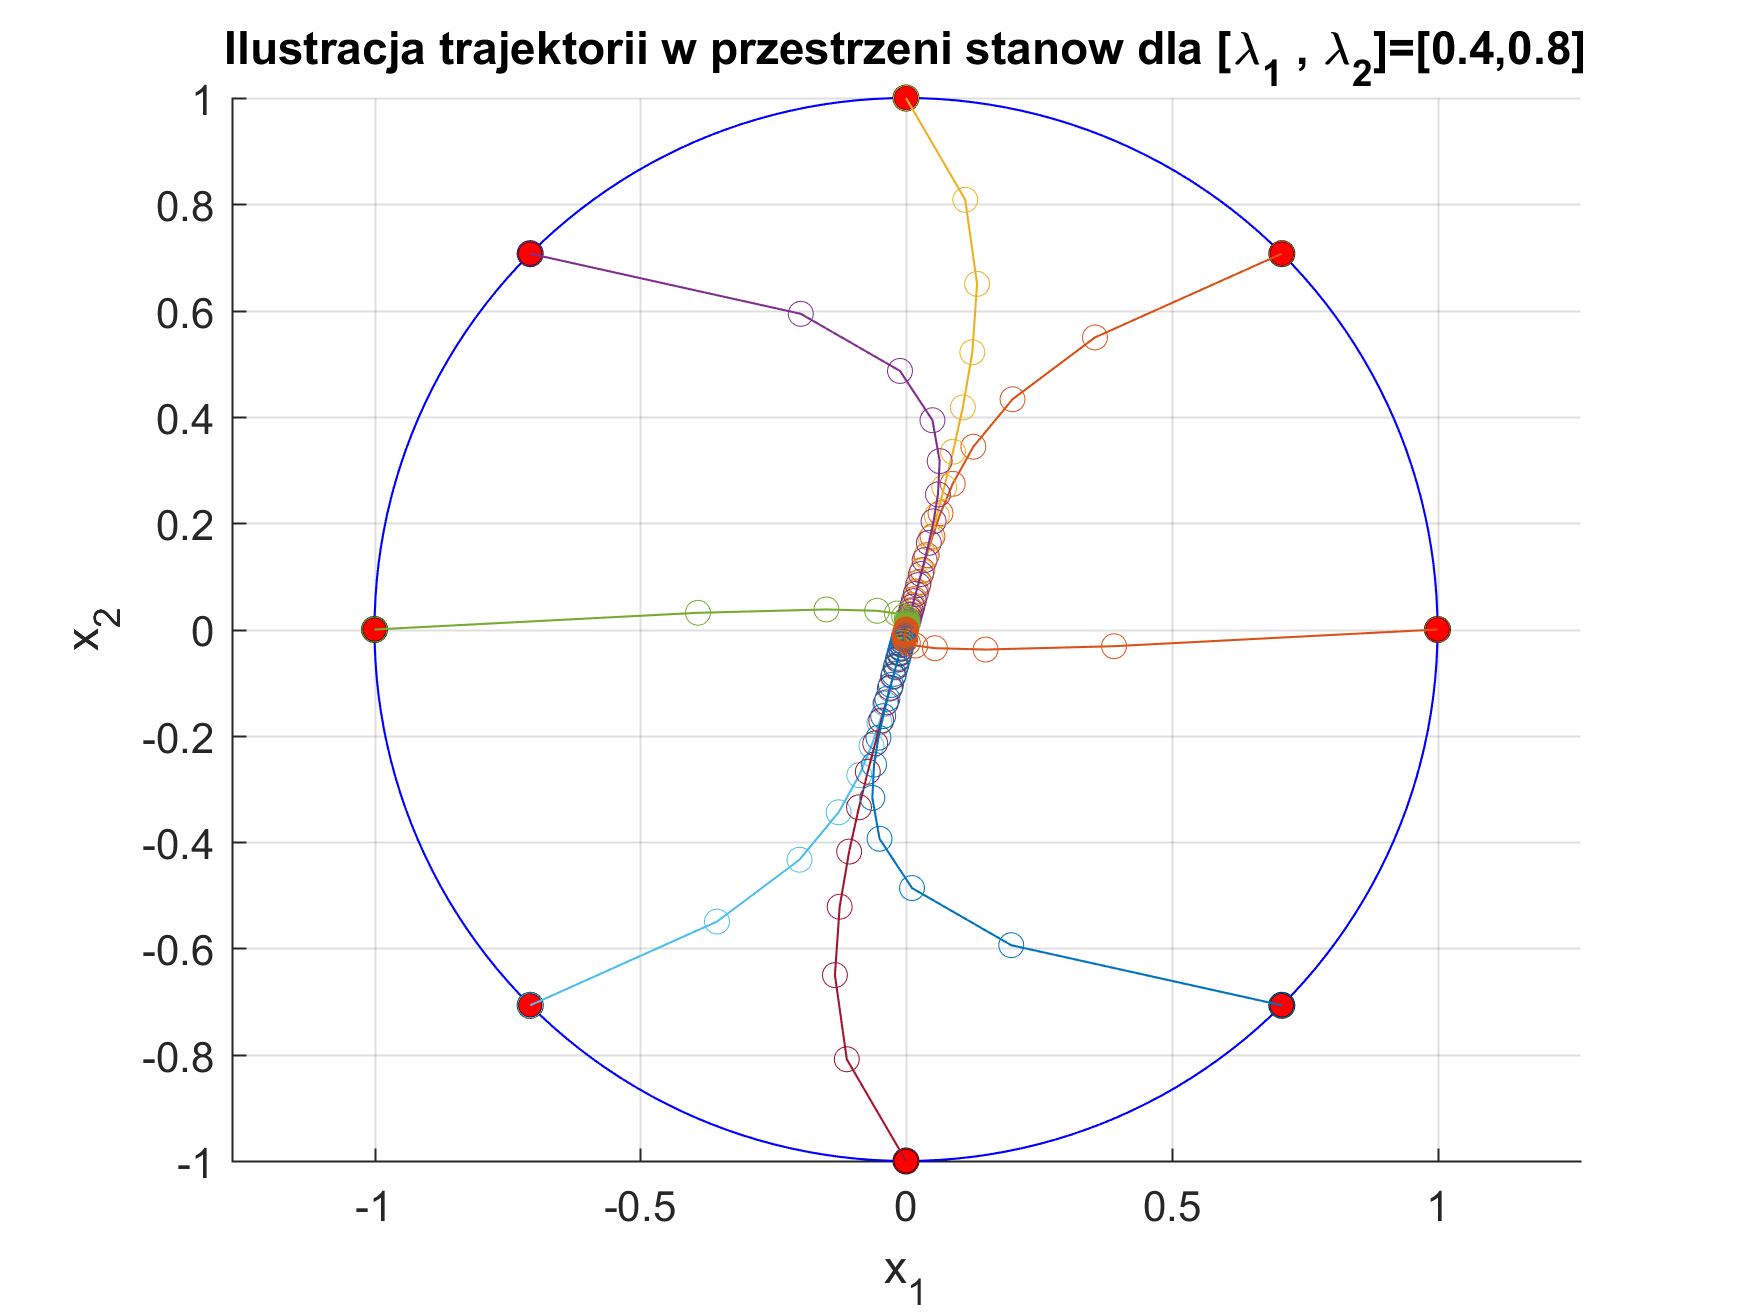
\includegraphics[width=\textwidth]{portret_fazowy_4_8.png}
    \end{subfigure}
    \begin{subfigure}{0.48\textwidth}
        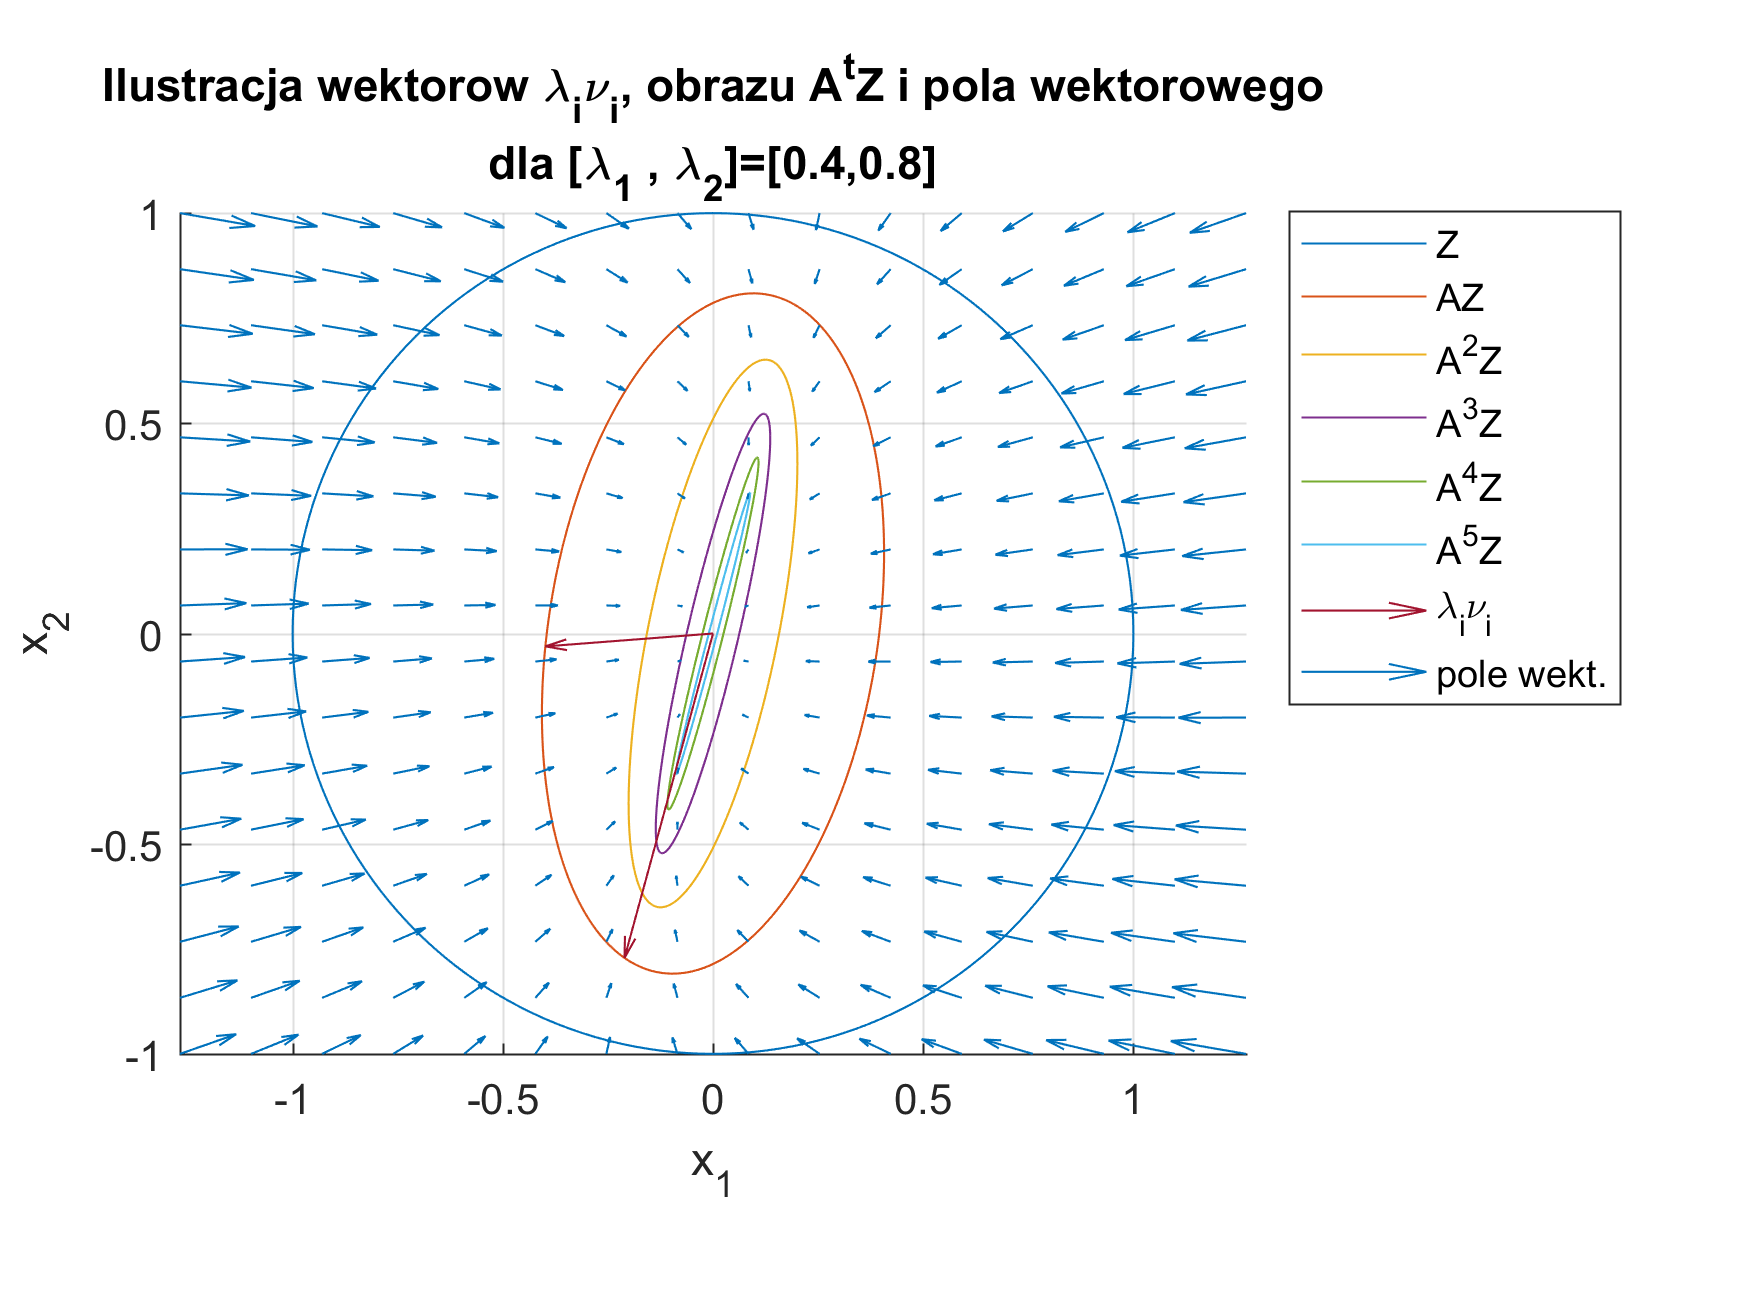
\includegraphics[width=\textwidth]{pole_wektorowe_4_8.png}
    \end{subfigure}
    \caption{Warto\'sci własne $[ \lambda_1, \lambda_2 ]= [ 0.4, 0.8 ]$}
    \label{fig::4i8}
\end{figure}
\begin{figure}[H]
    \centering
    \begin{subfigure}{0.44\textwidth}
        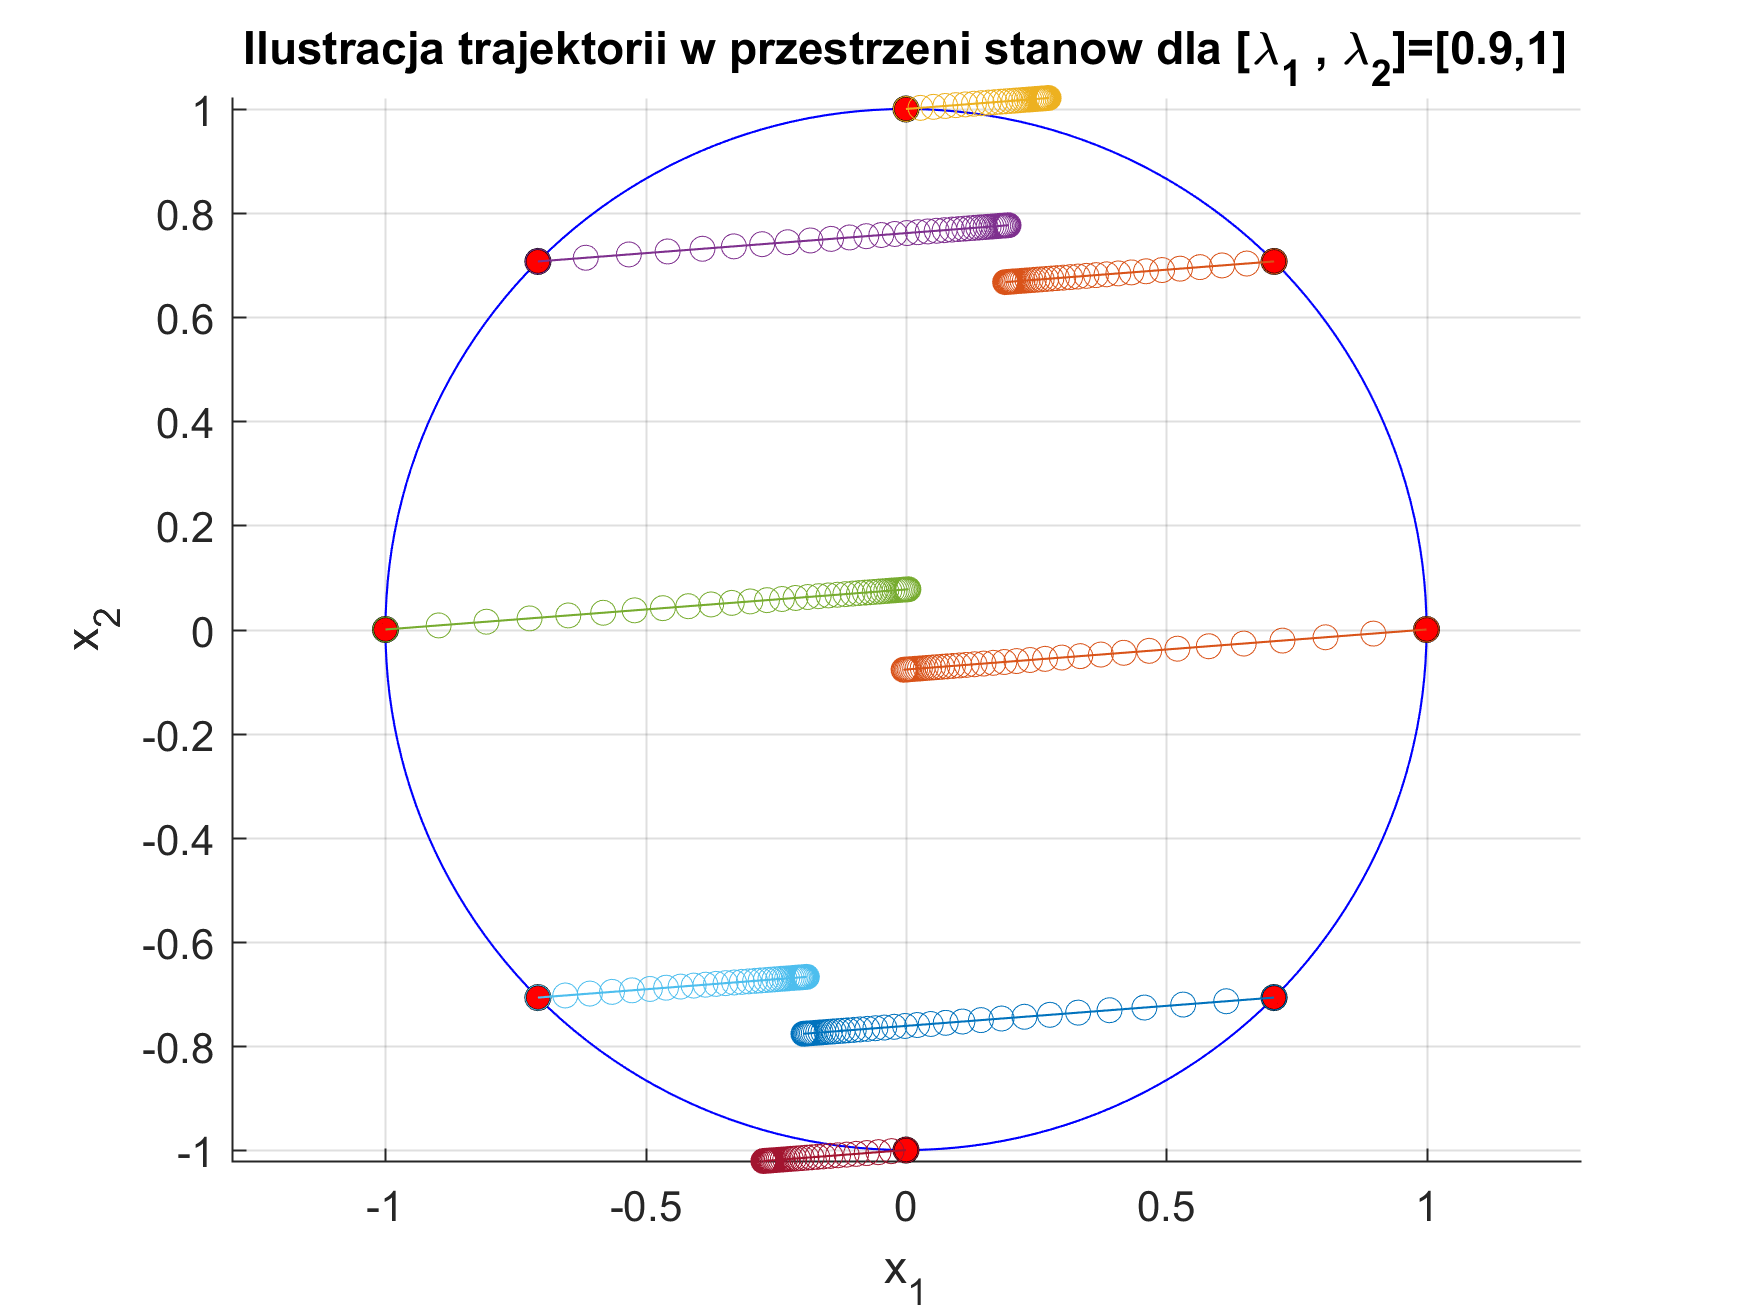
\includegraphics[width=\textwidth]{portret_fazowy_9_10.png}
    \end{subfigure}
    \begin{subfigure}{0.48\textwidth}
        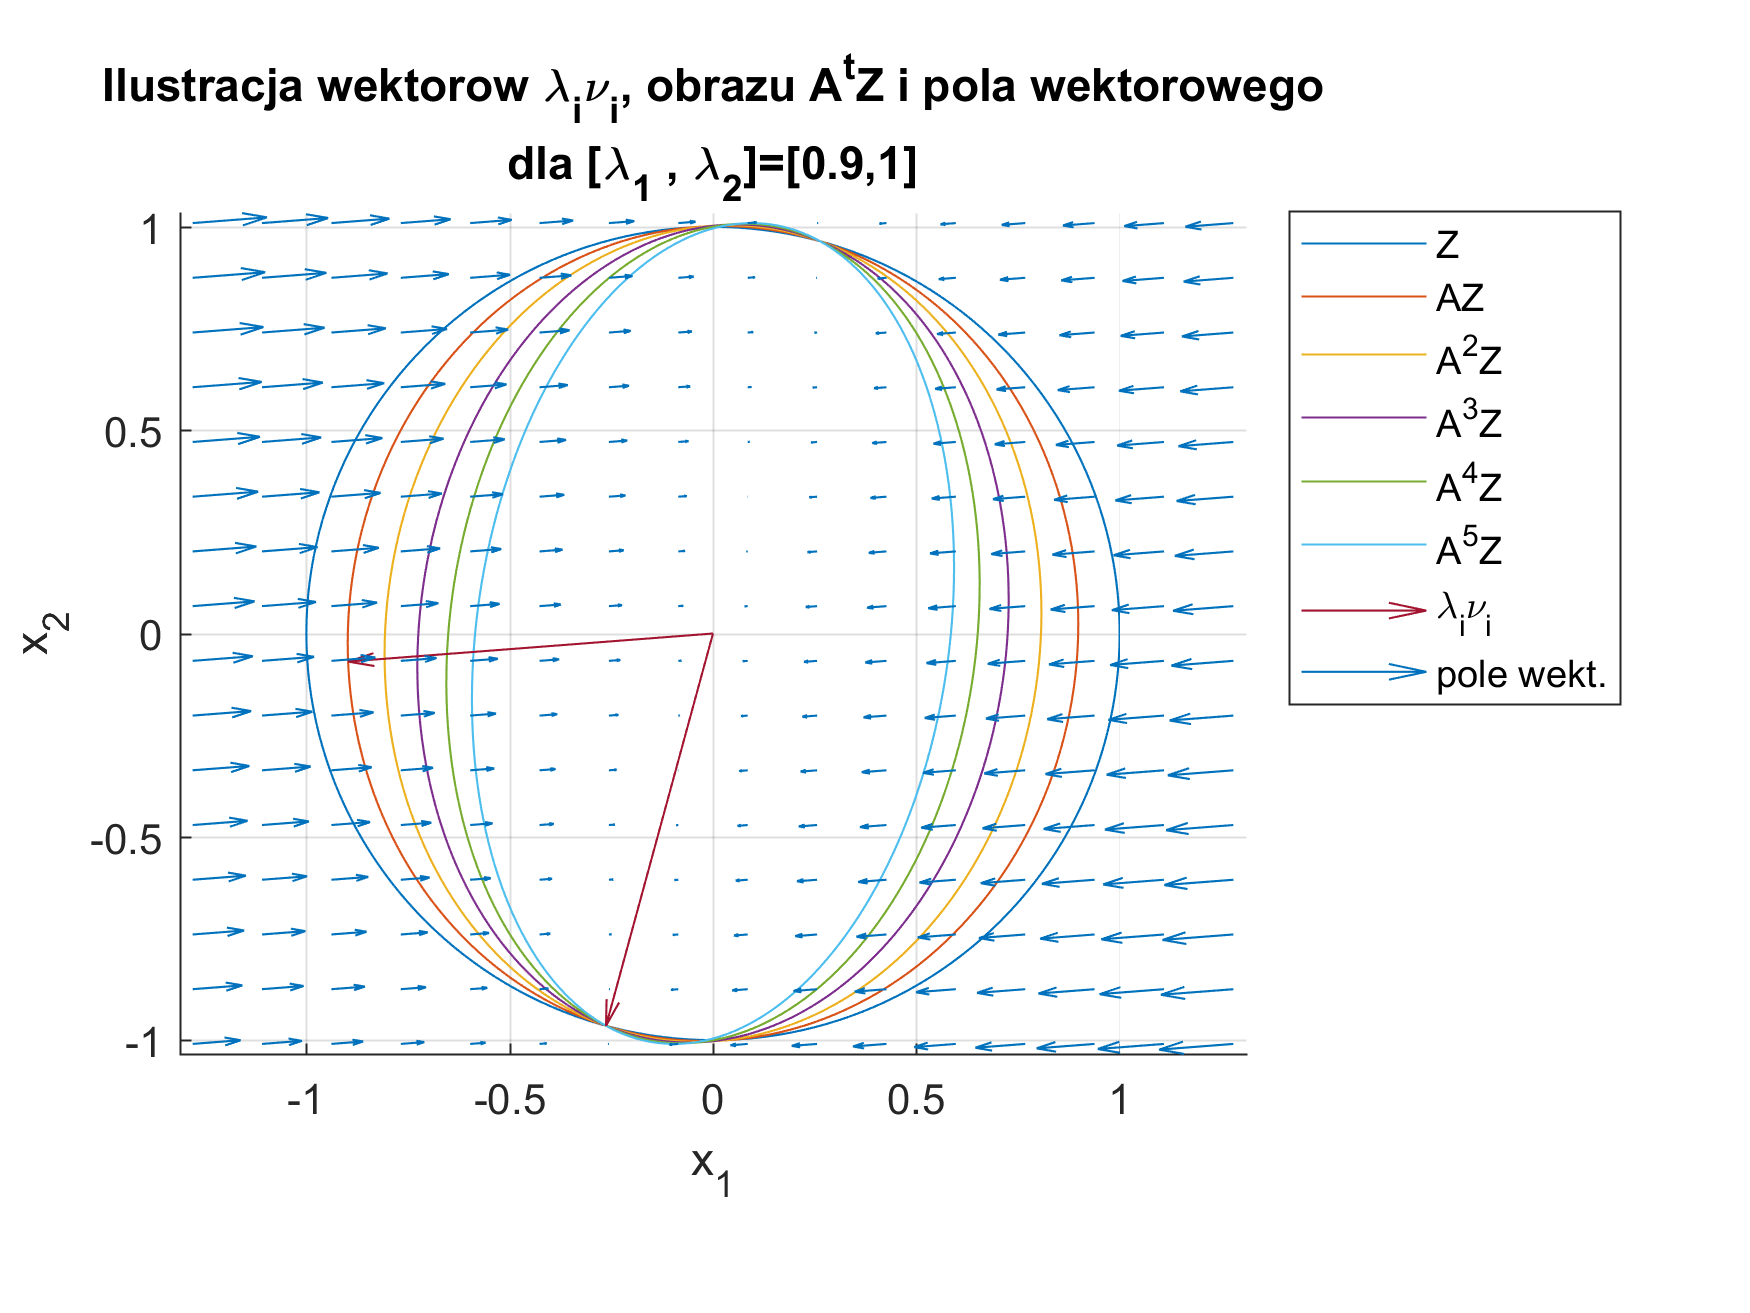
\includegraphics[width=\textwidth]{pole_wektorowe_9_10.png}
    \end{subfigure}
    \caption{Warto\'sci własne $[ \lambda_1, \lambda_2 ]= [ 0.9, 1 ]$}
    \label{fig::9i10}
\end{figure}
\begin{figure}[H]
    \centering
    \begin{subfigure}{0.44\textwidth}
        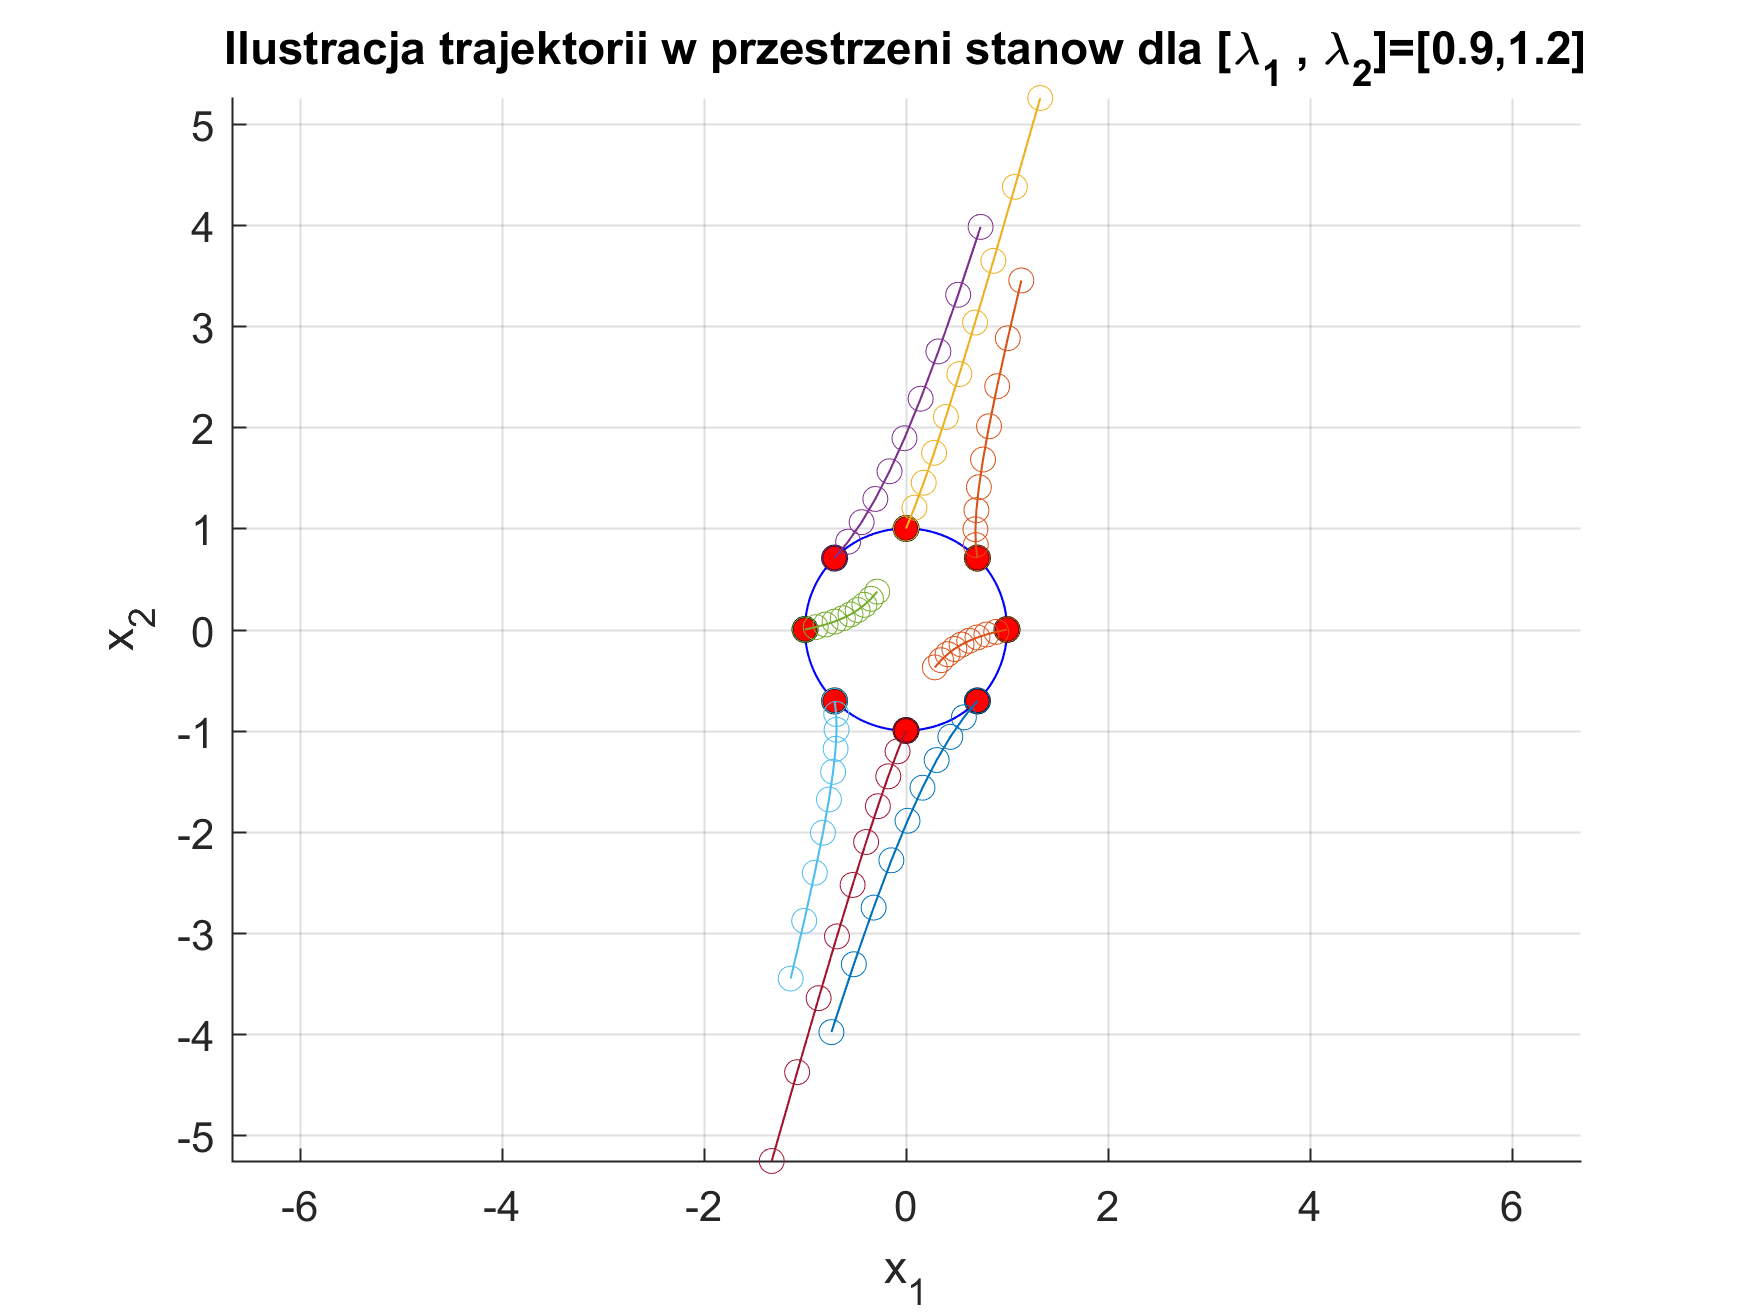
\includegraphics[width=\textwidth]{portret_fazowy_9_12.png}
    \end{subfigure}
    \begin{subfigure}{0.48\textwidth}
        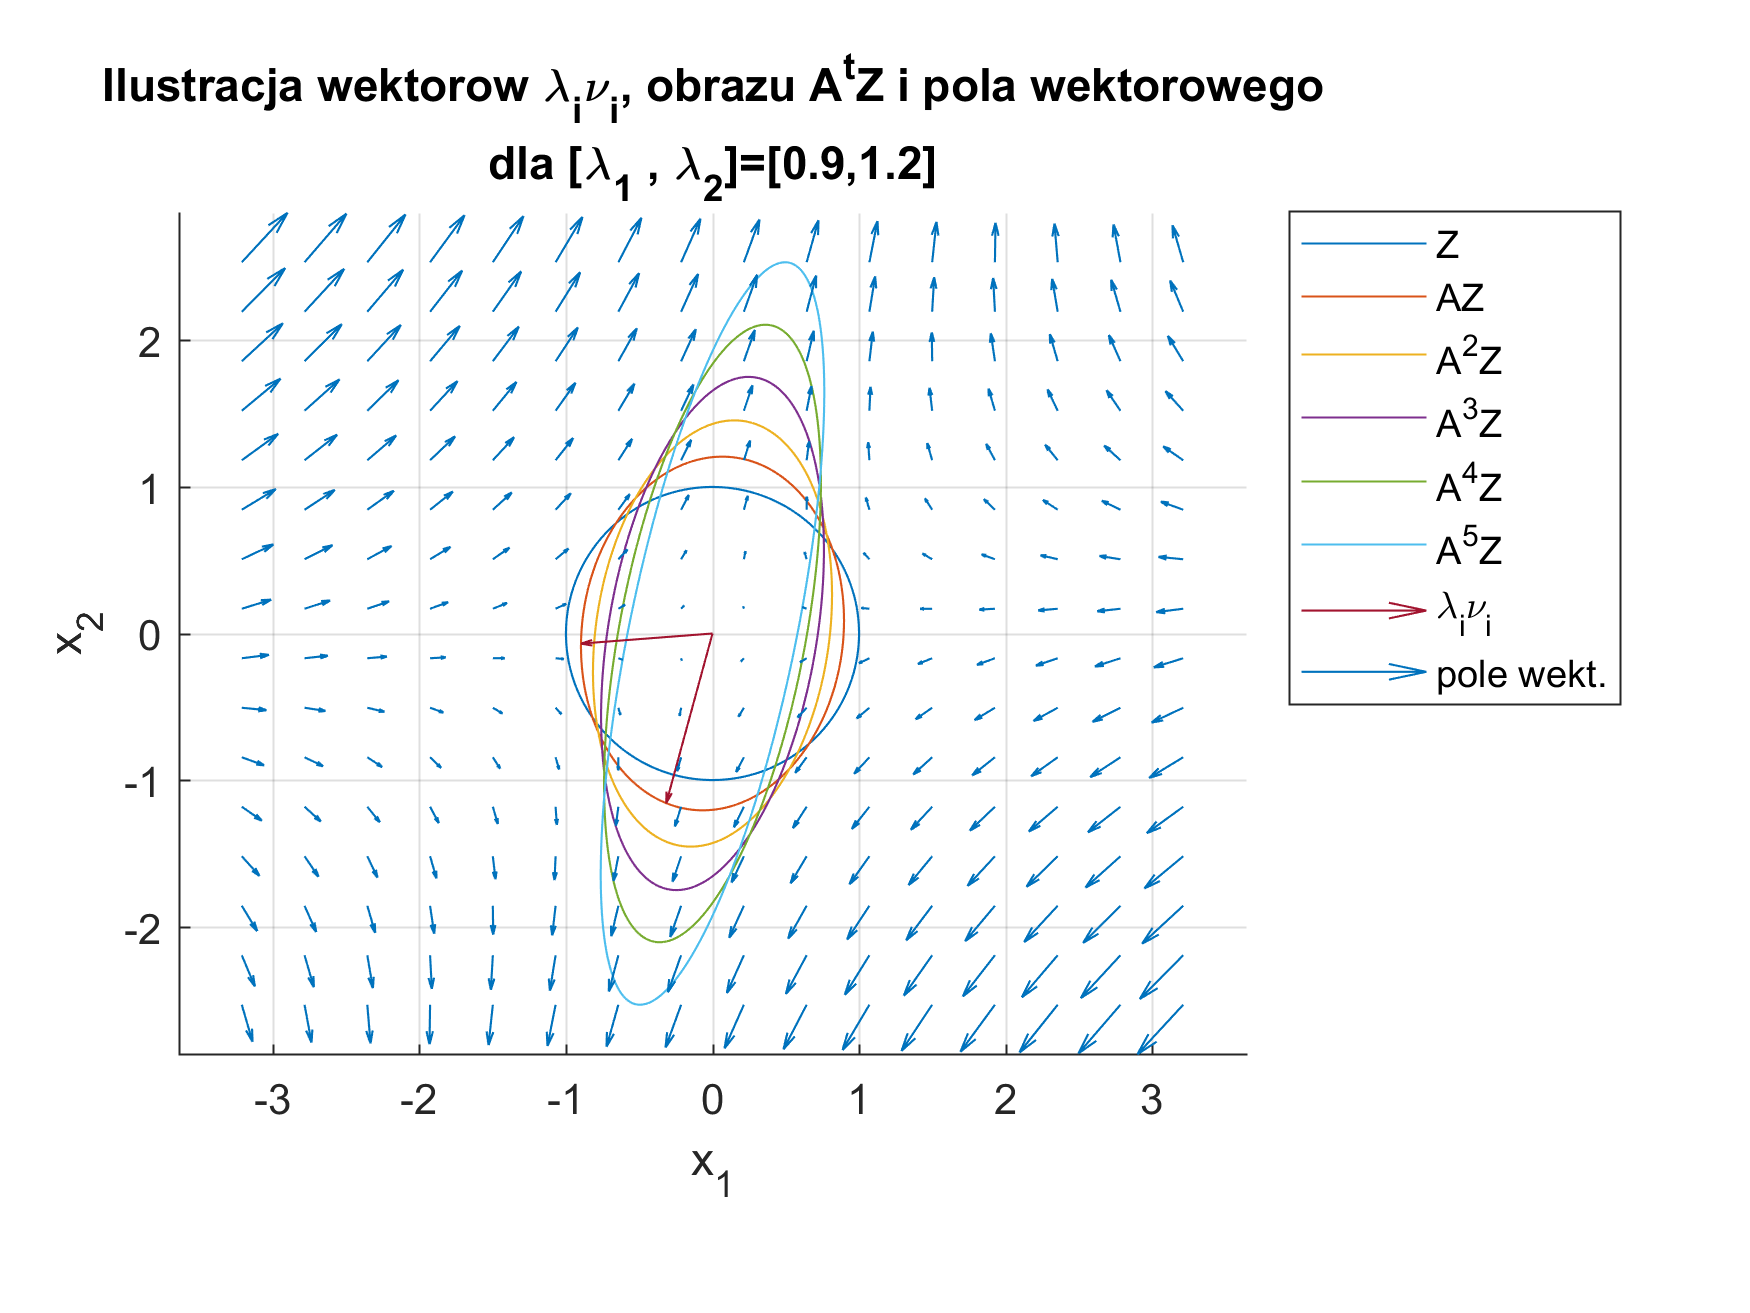
\includegraphics[width=\textwidth]{pole_wektorowe_9_12.png}
    \end{subfigure}
    \caption{Warto\'sci własne $[ \lambda_1, \lambda_2 ]= [ 0.9, 1.2 ]$}
    \label{fig::9i12}
\end{figure}

\begin{figure}[H]
    \centering
    \begin{subfigure}{0.44\textwidth}
        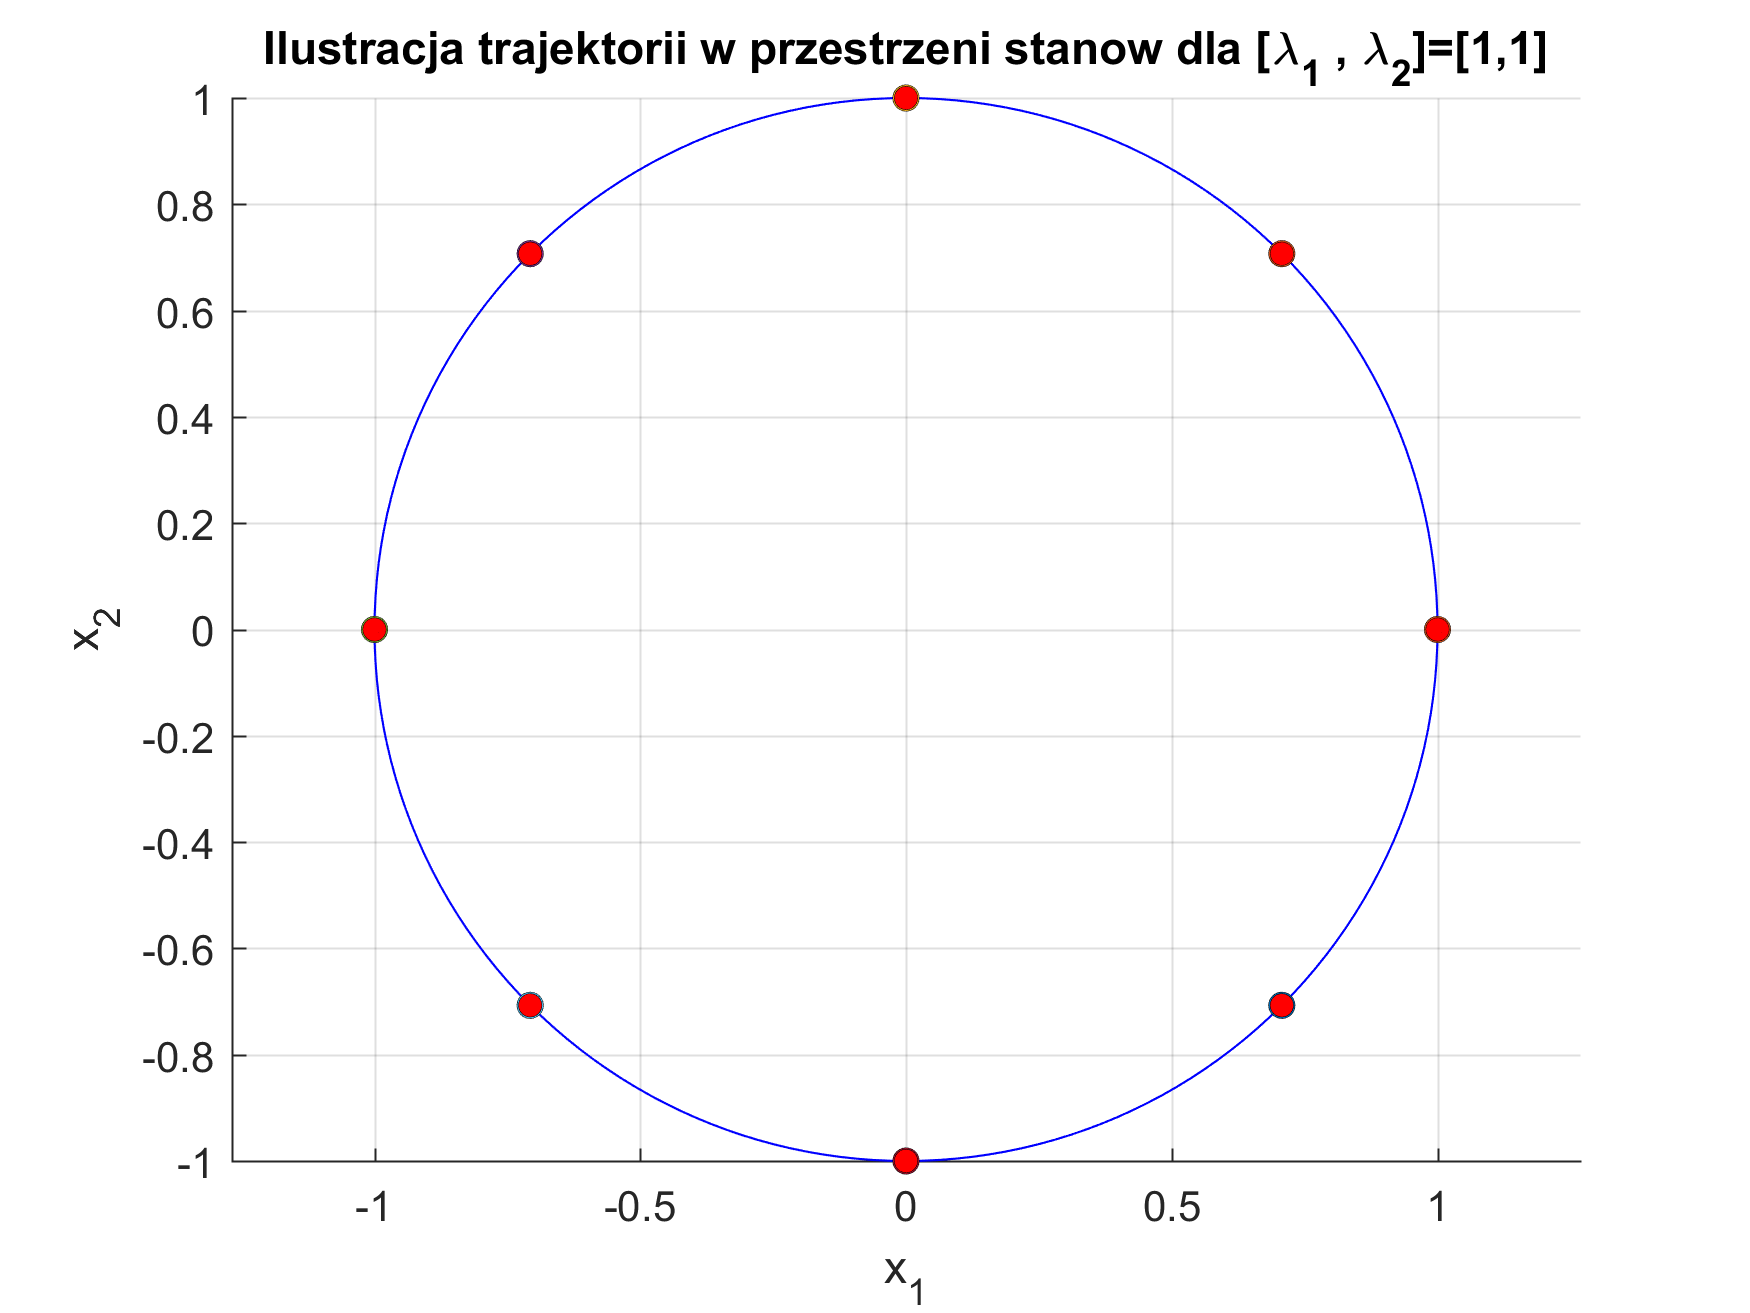
\includegraphics[width=\textwidth]{portret_fazowy_10_10.png}
    \end{subfigure}
    \begin{subfigure}{0.48\textwidth}
        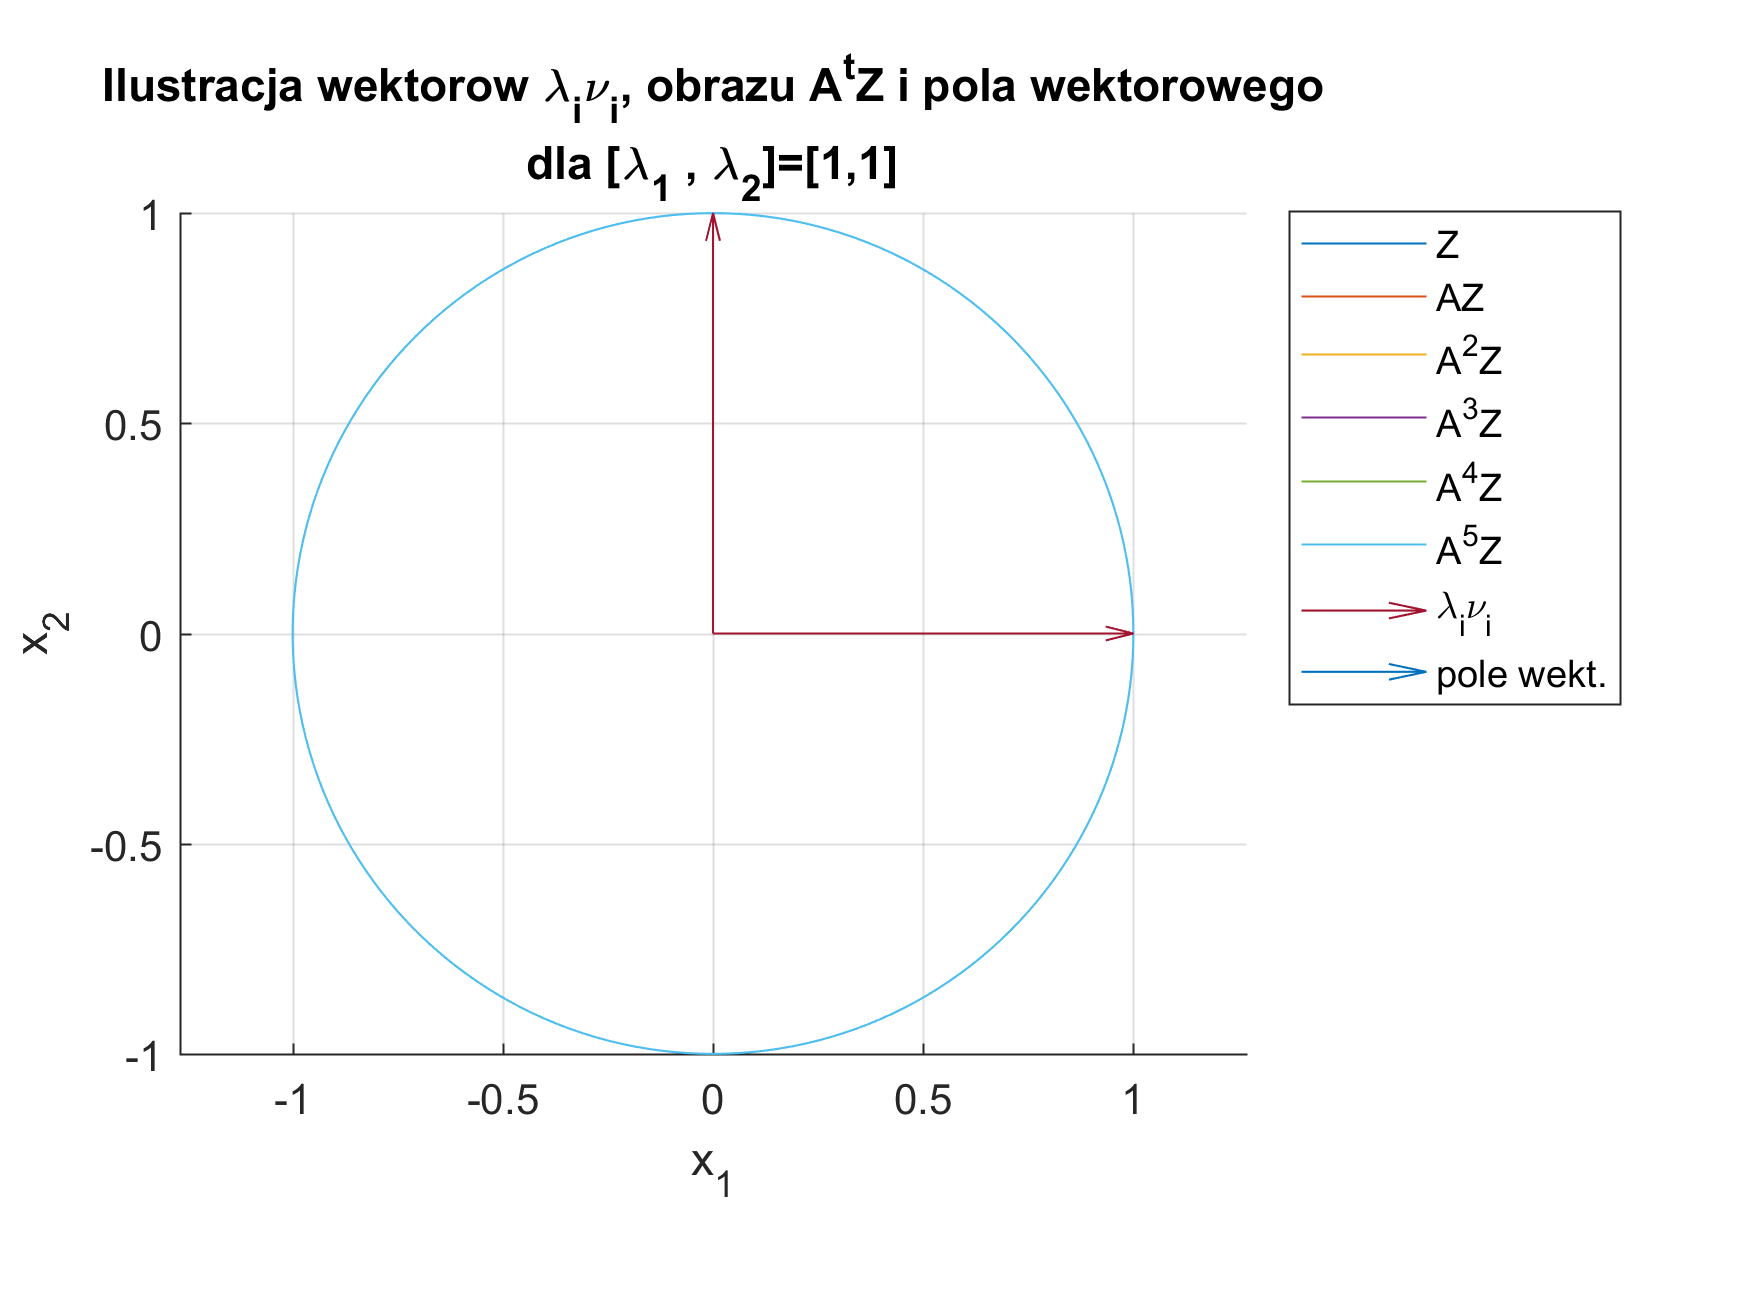
\includegraphics[width=\textwidth]{pole_wektorowe_10_10.png}
    \end{subfigure}
    \caption{Warto\'sci własne $[ \lambda_1, \lambda_2 ]= [ 1, 1 ]$}
    \label{fig::10i10}
\end{figure}
\begin{figure}[H]
    \centering
    \begin{subfigure}{0.44\textwidth}
        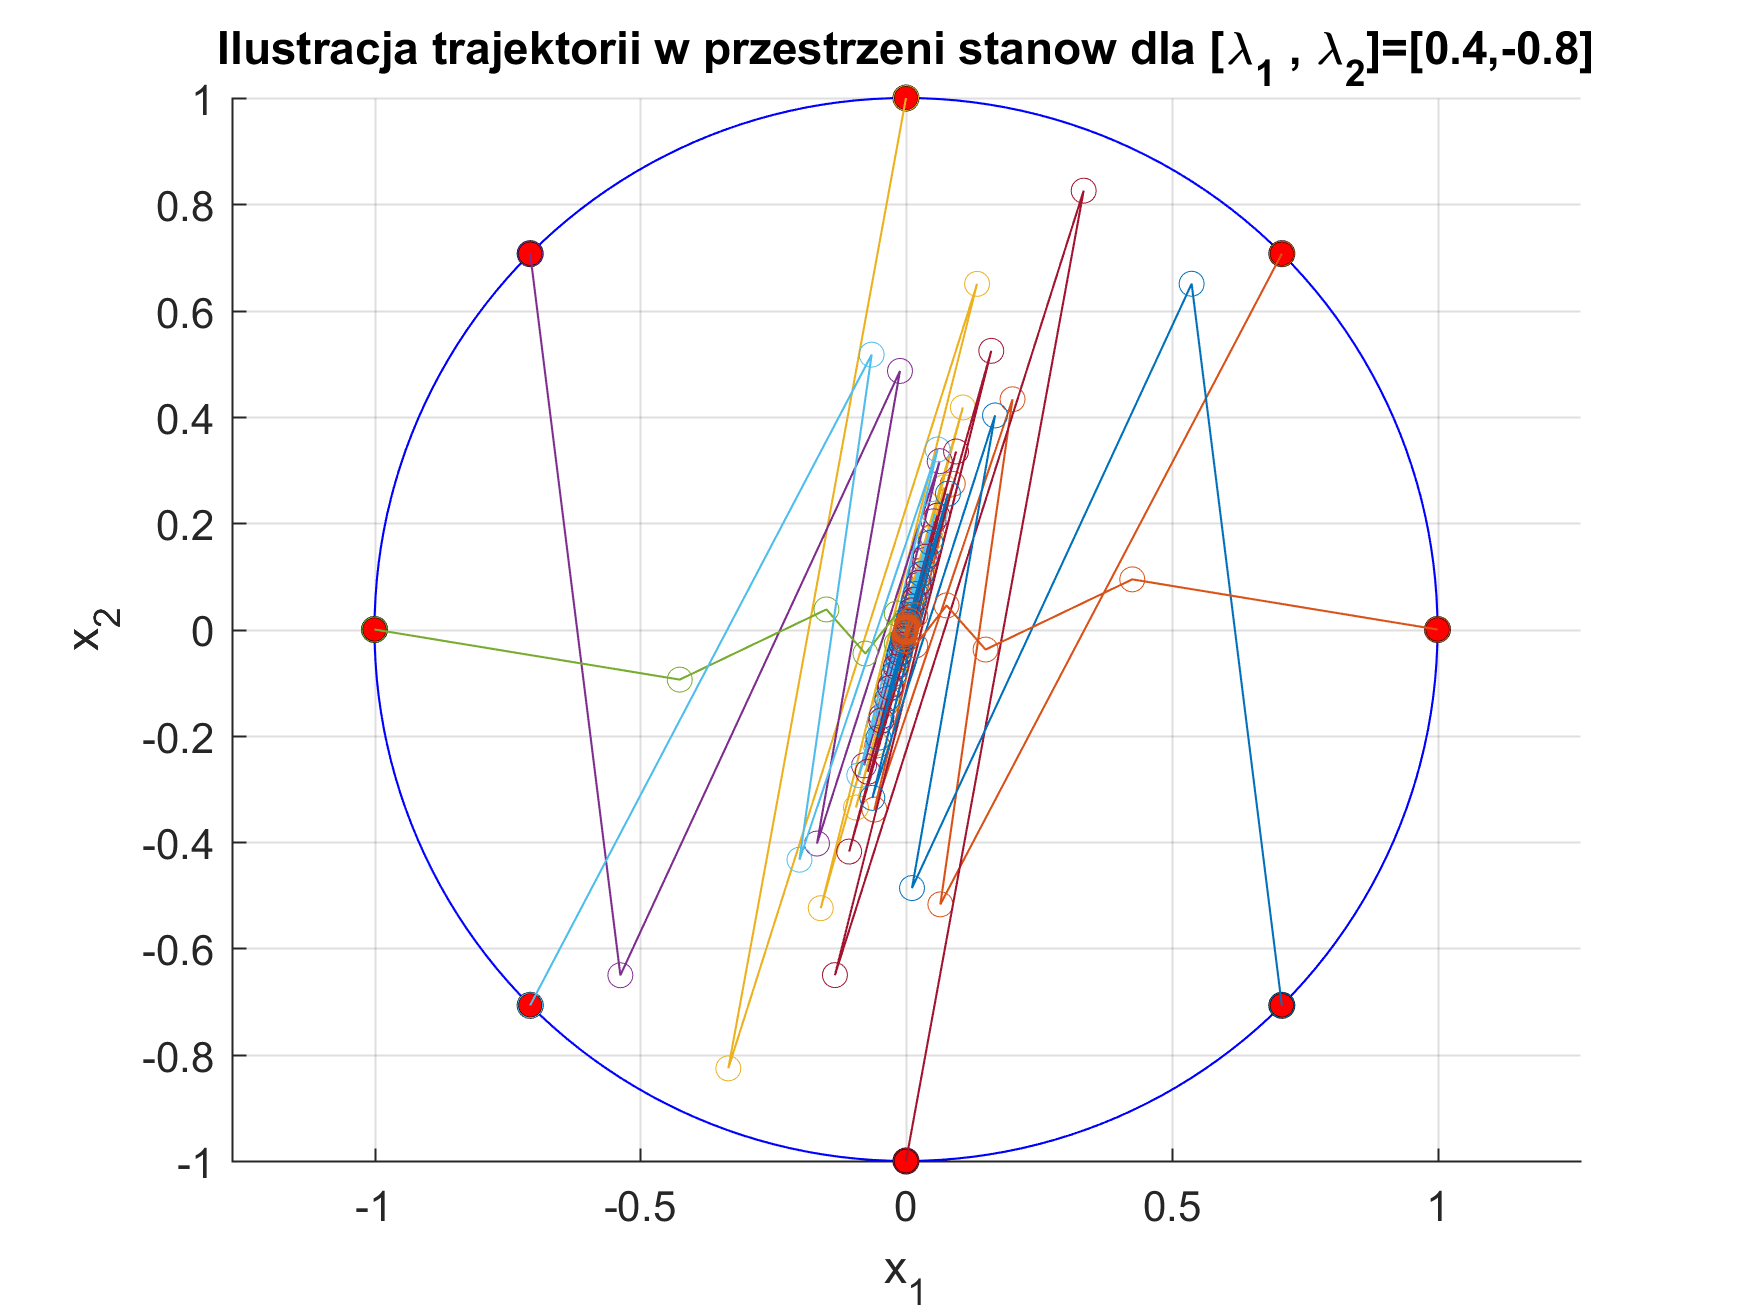
\includegraphics[width=\textwidth]{portret_fazowy_4_-8.png}
    \end{subfigure}
    \begin{subfigure}{0.48\textwidth}
        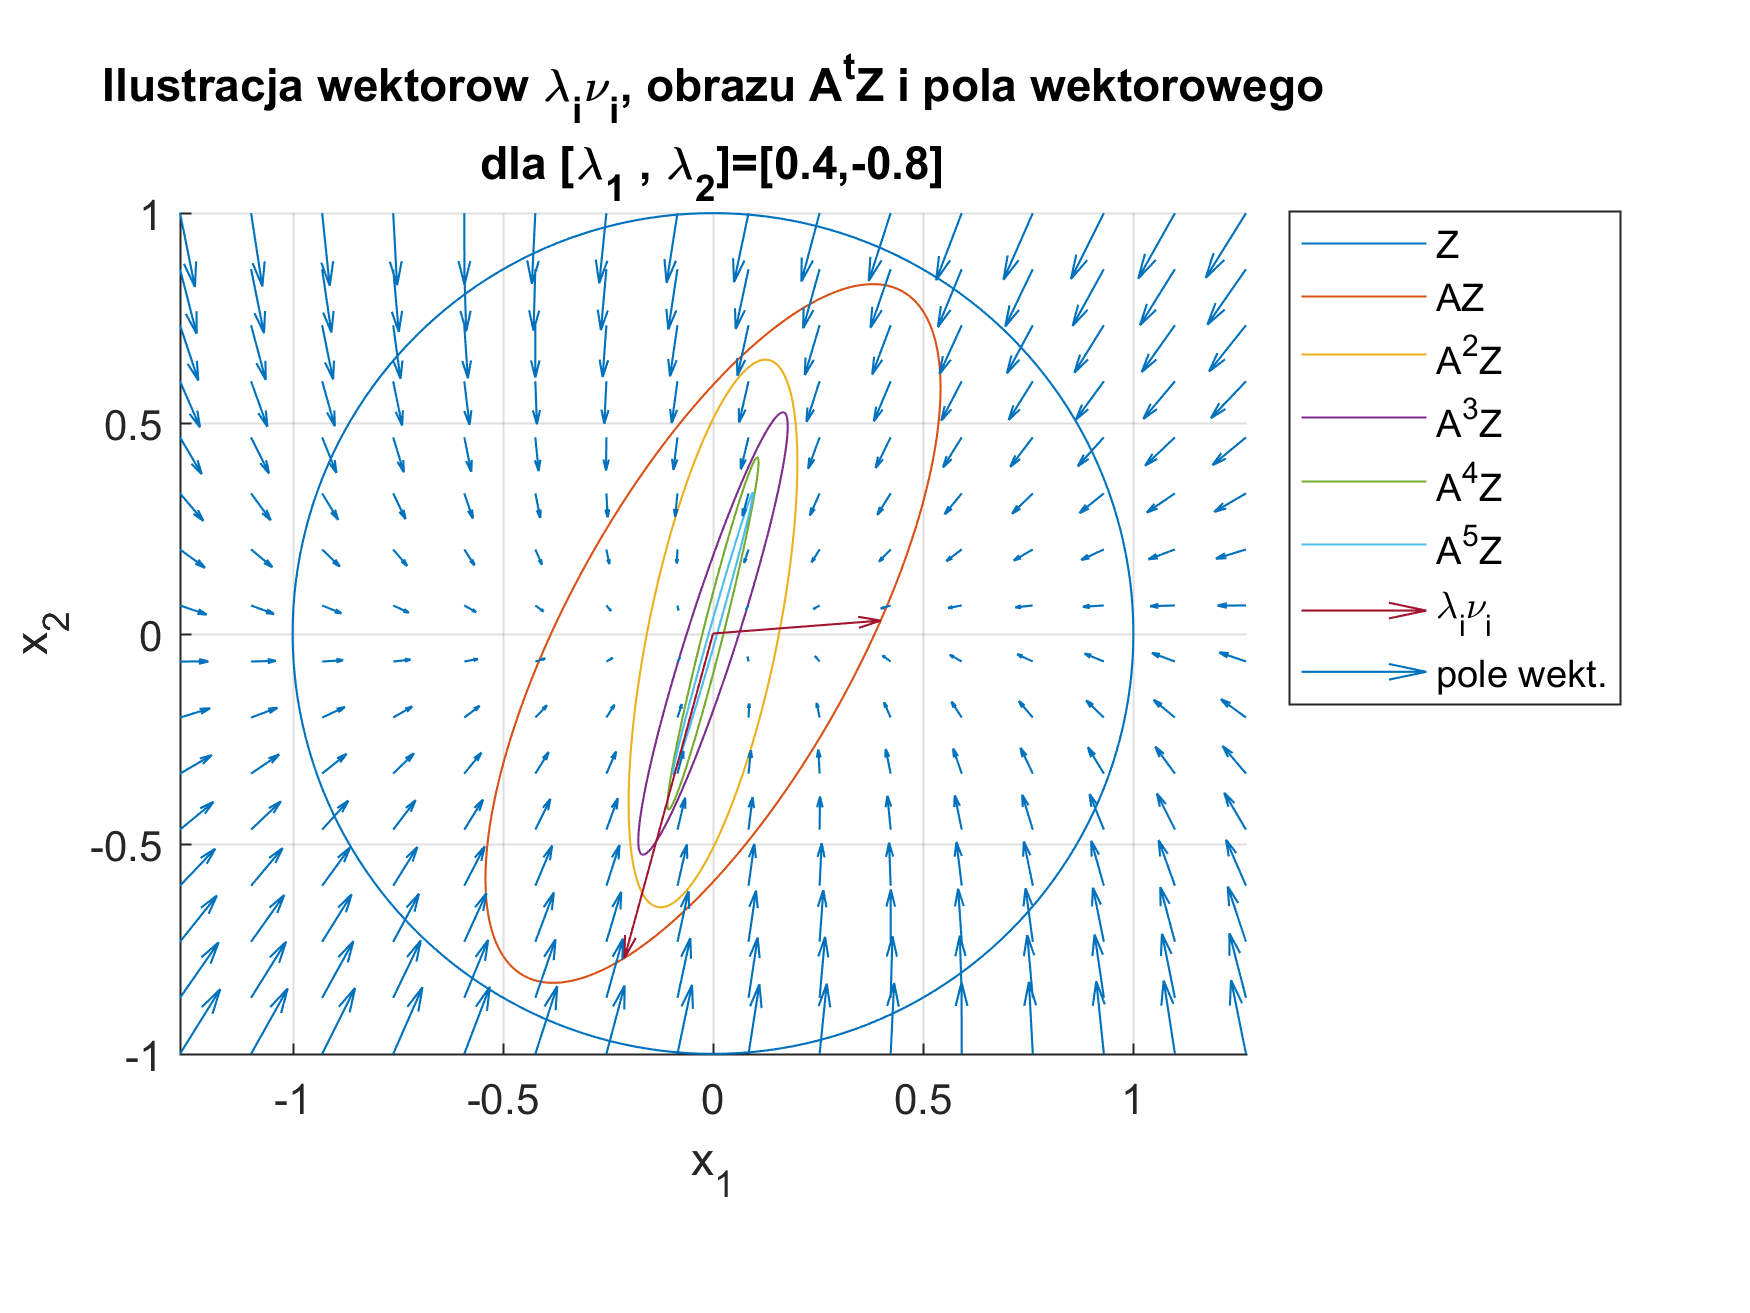
\includegraphics[width=\textwidth]{pole_wektorowe_4_-8.png}
    \end{subfigure}
    \caption{Warto\'sci własne $[ \lambda_1, \lambda_2 ]= [ 0.4, -0.8 ]$}
    \label{fig::4i-8}
\end{figure}
\begin{figure}[H]
    \centering
    \begin{subfigure}{0.44\textwidth}
        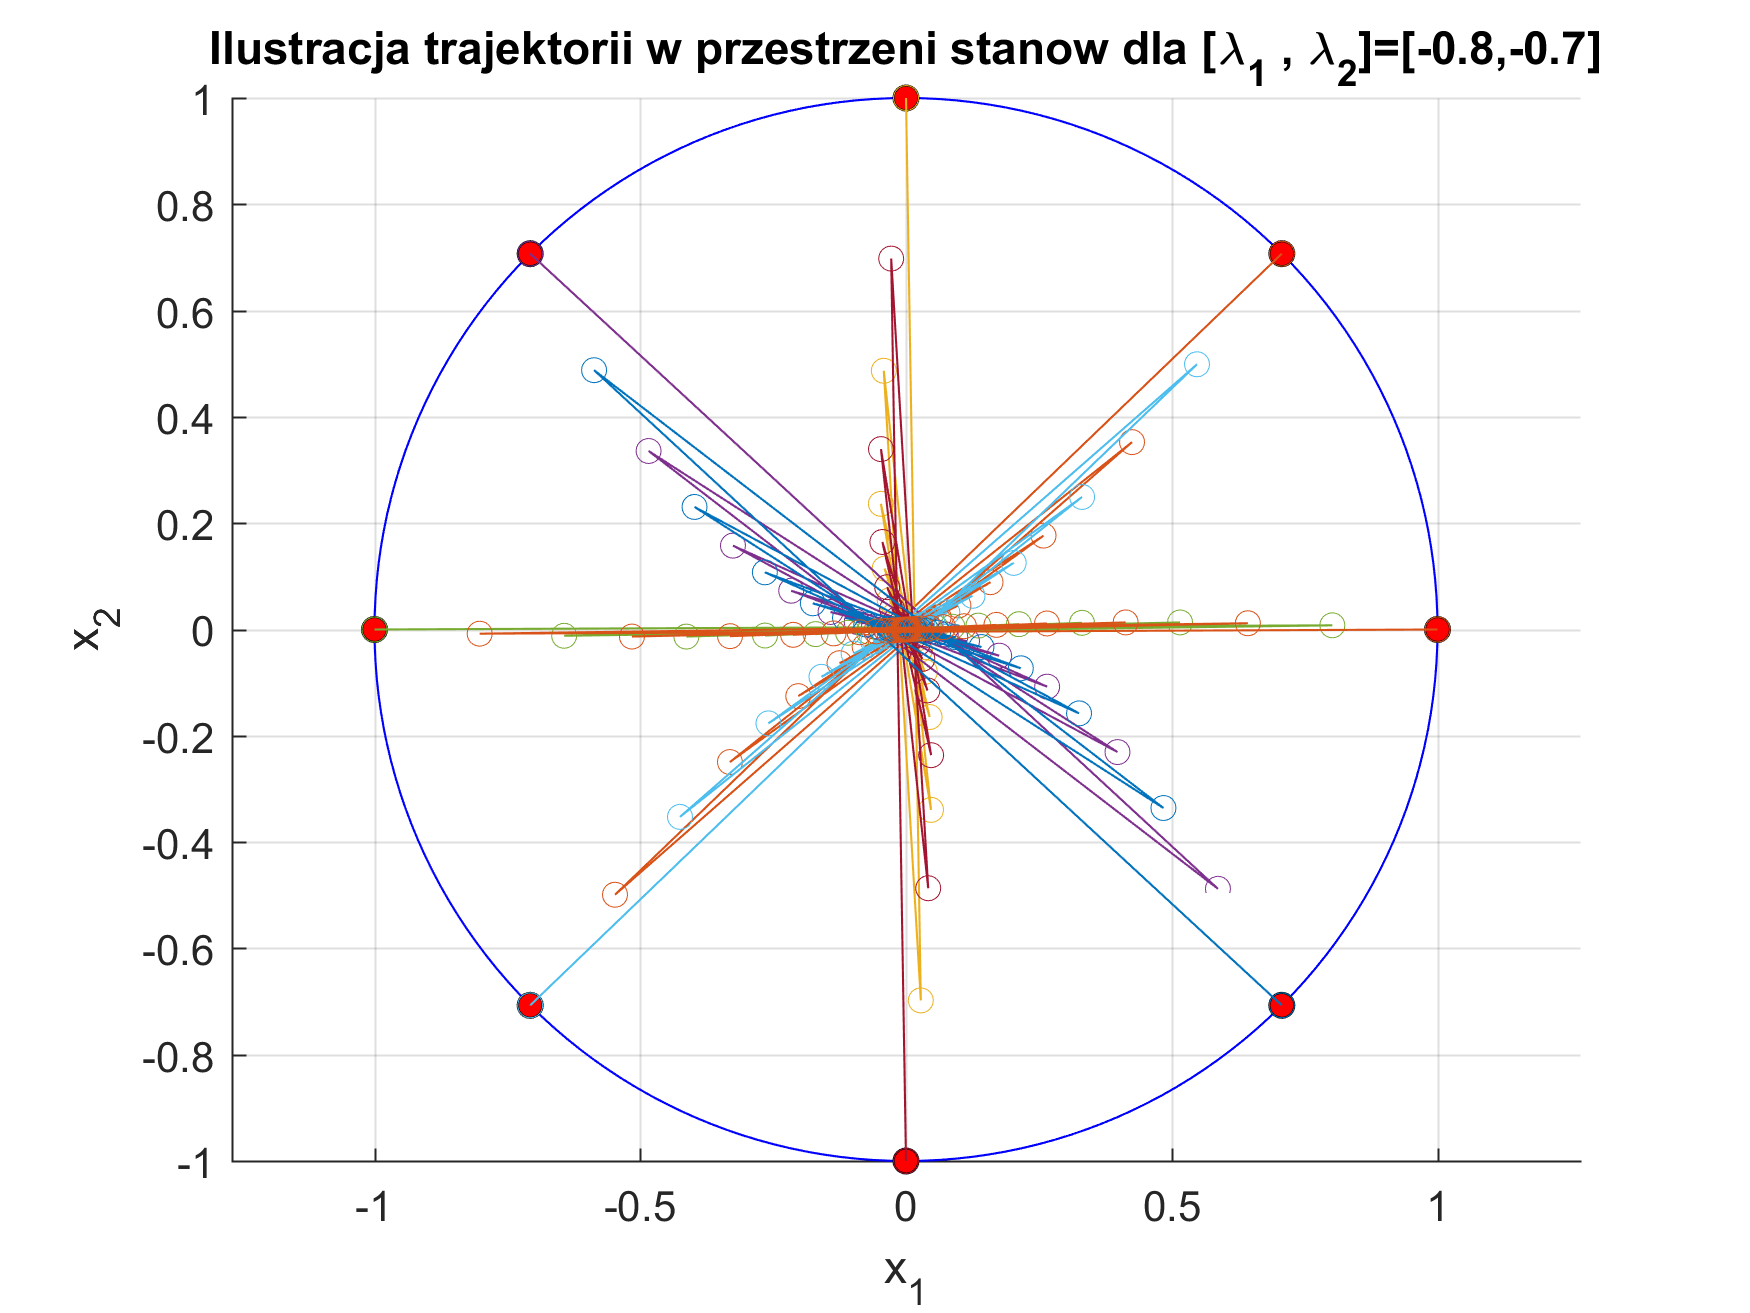
\includegraphics[width=\textwidth]{portret_fazowy_-8_-7.png}
    \end{subfigure}
    \begin{subfigure}{0.48\textwidth}
        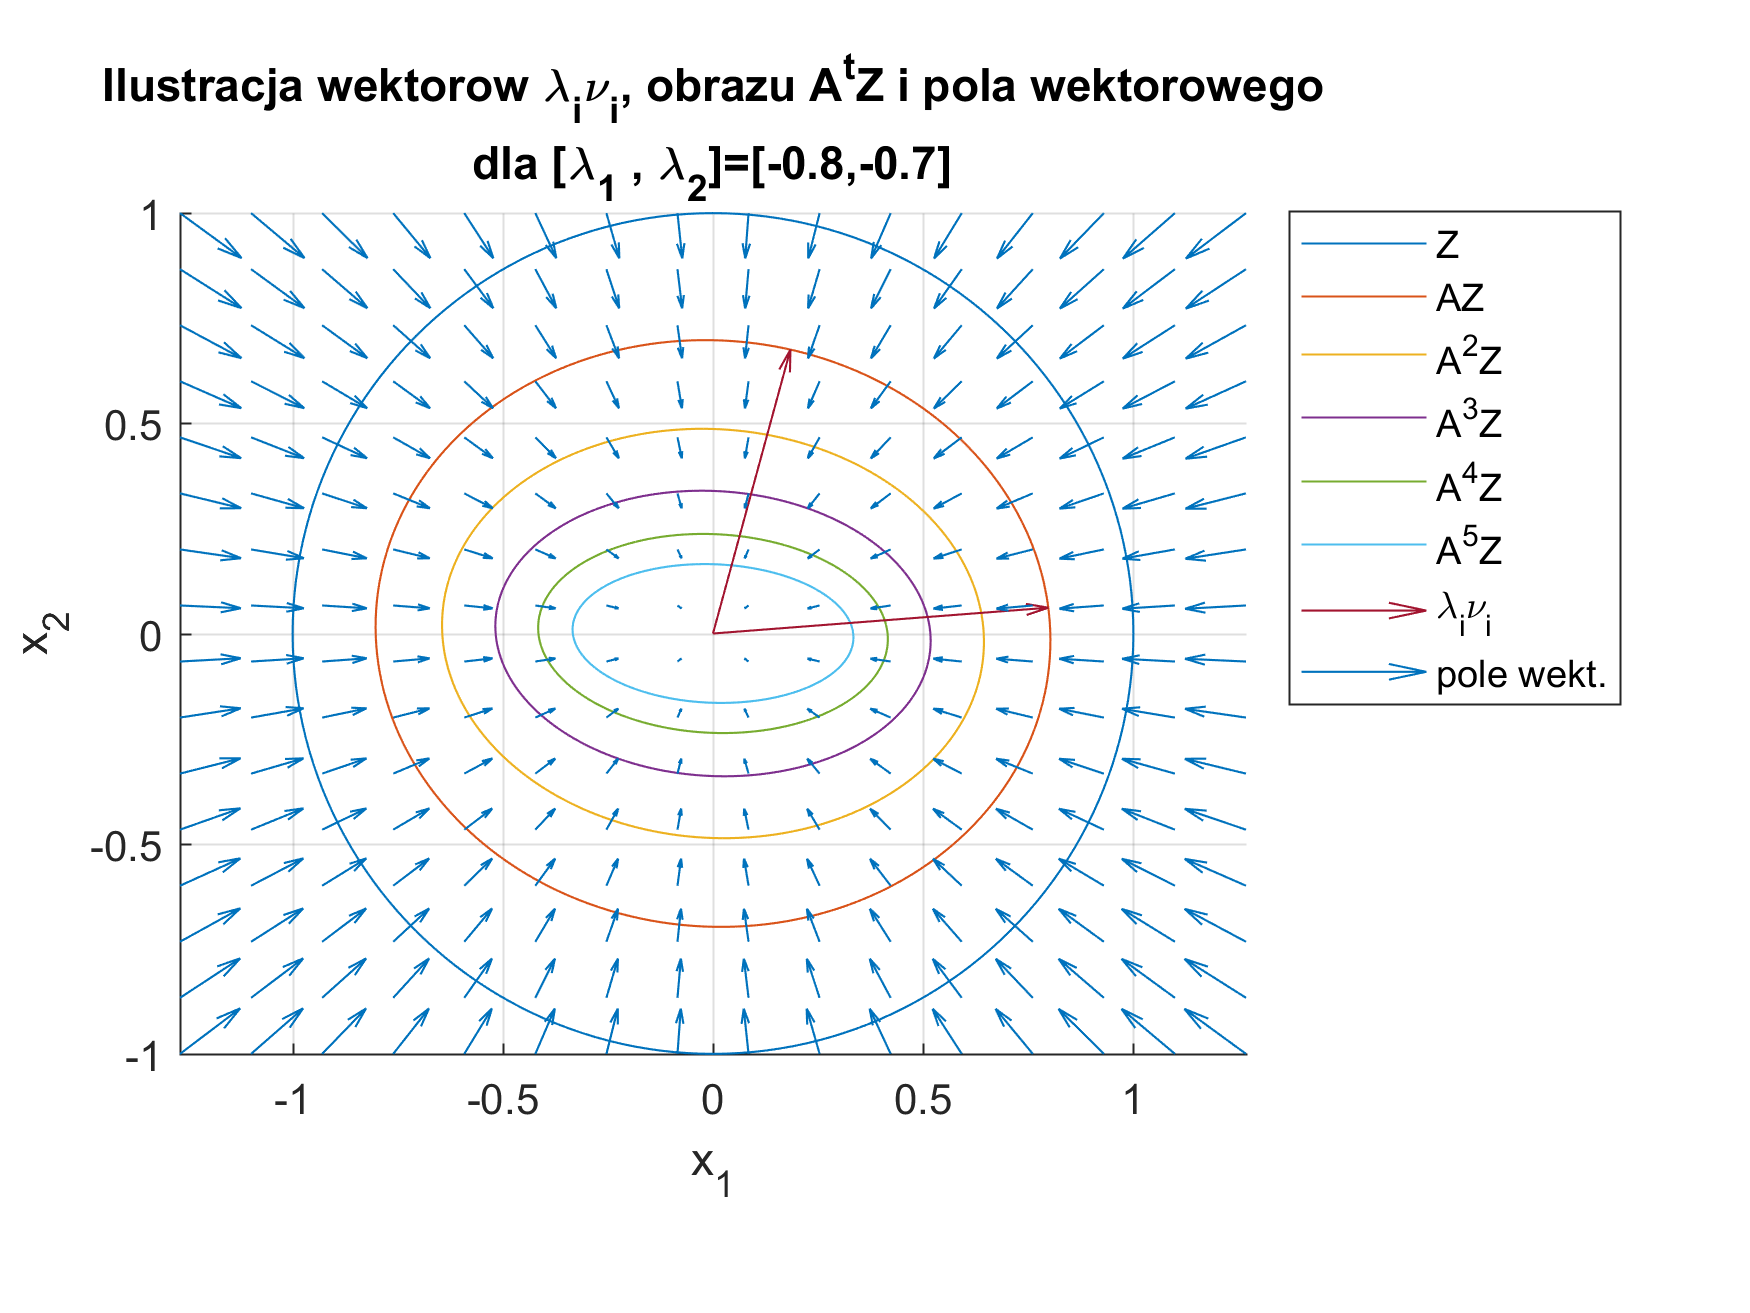
\includegraphics[width=\textwidth]{pole_wektorowe_-8_-7.png}
    \end{subfigure}
    \caption{Warto\'sci własne $[ \lambda_1, \lambda_2 ]= [ -0.8, -0.7 ]$}
    \label{fig::-8i-7}
\end{figure}

\begin{figure}[H]
    \centering
    \begin{subfigure}{0.44\textwidth}
        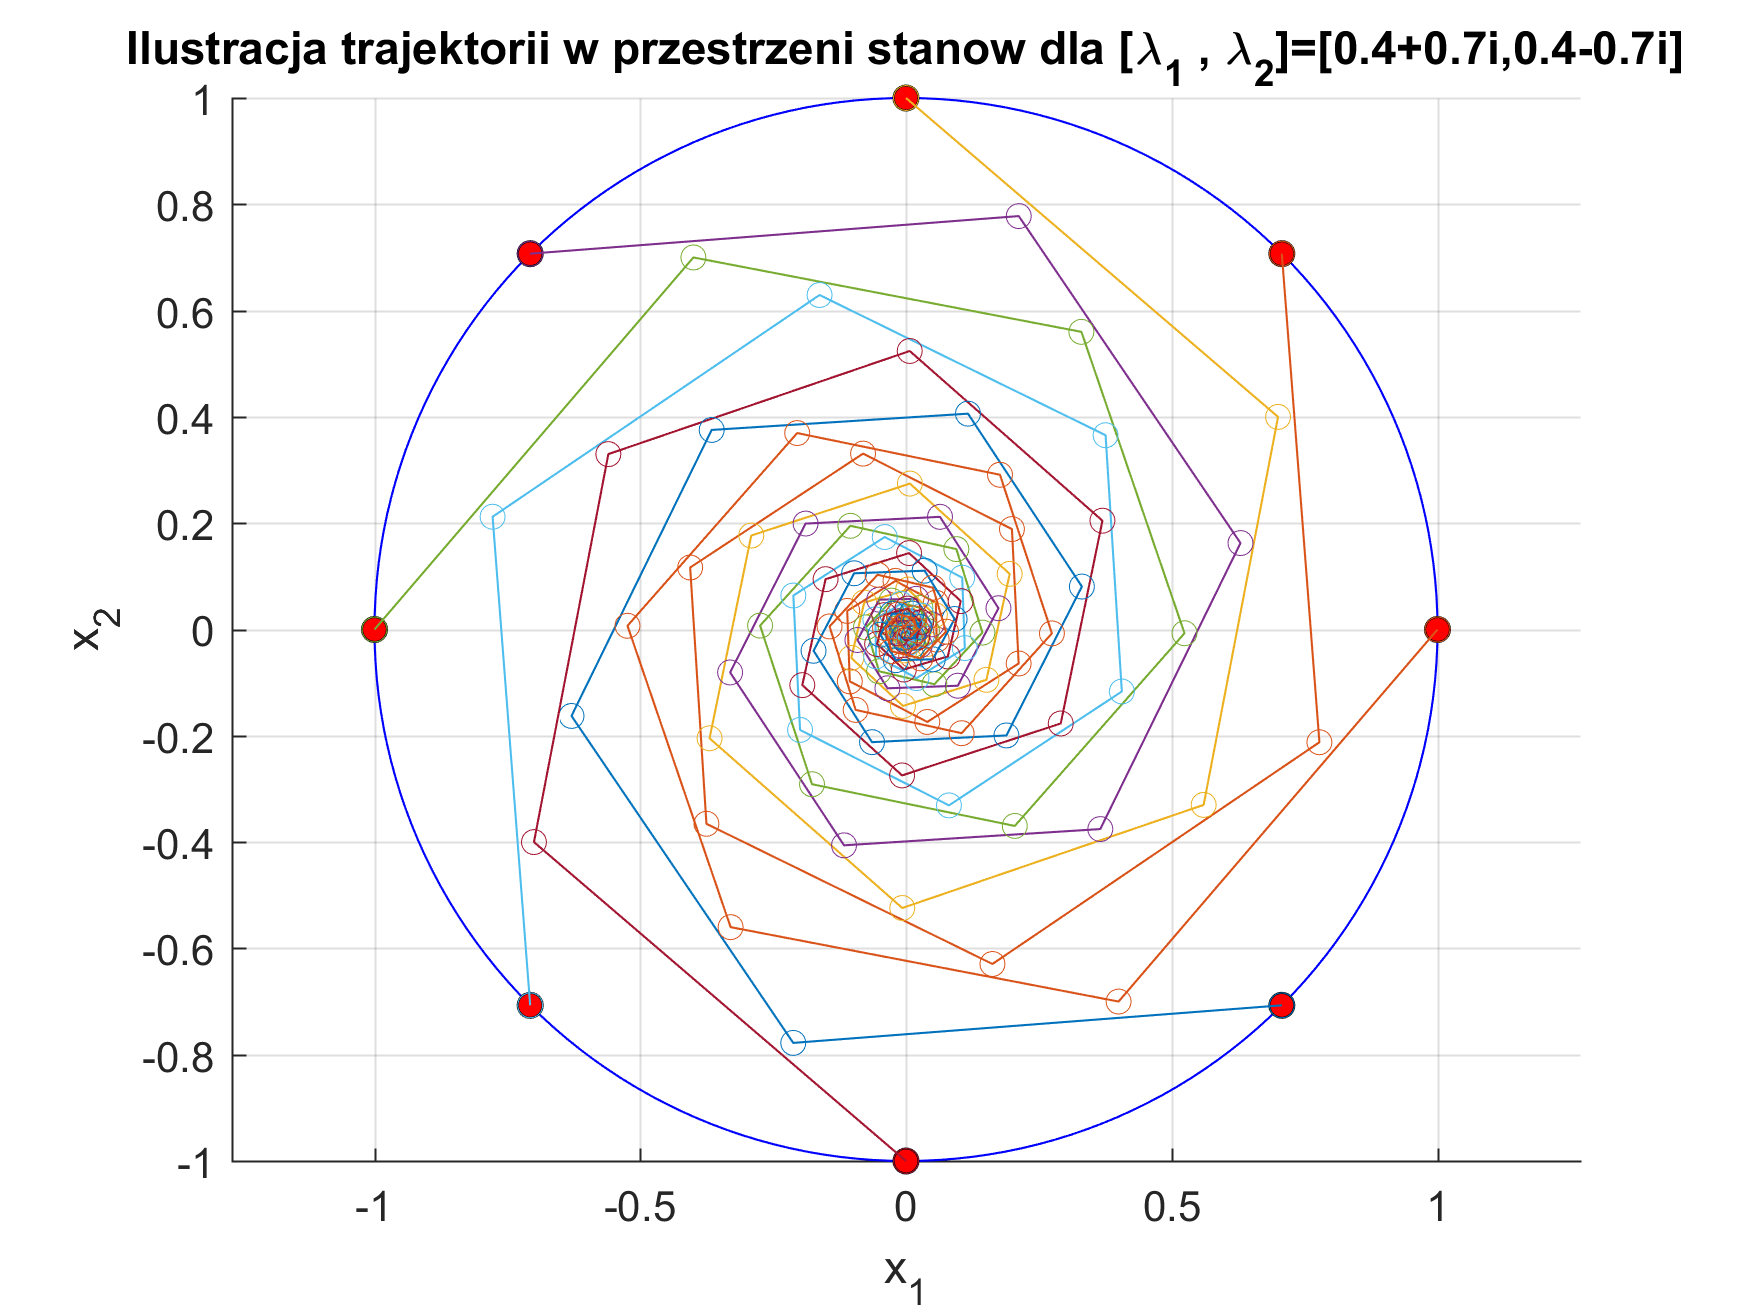
\includegraphics[width=\textwidth]{portret_fazowy_4+7i_4-7i.png}
    \end{subfigure}
    \begin{subfigure}{0.48\textwidth}
        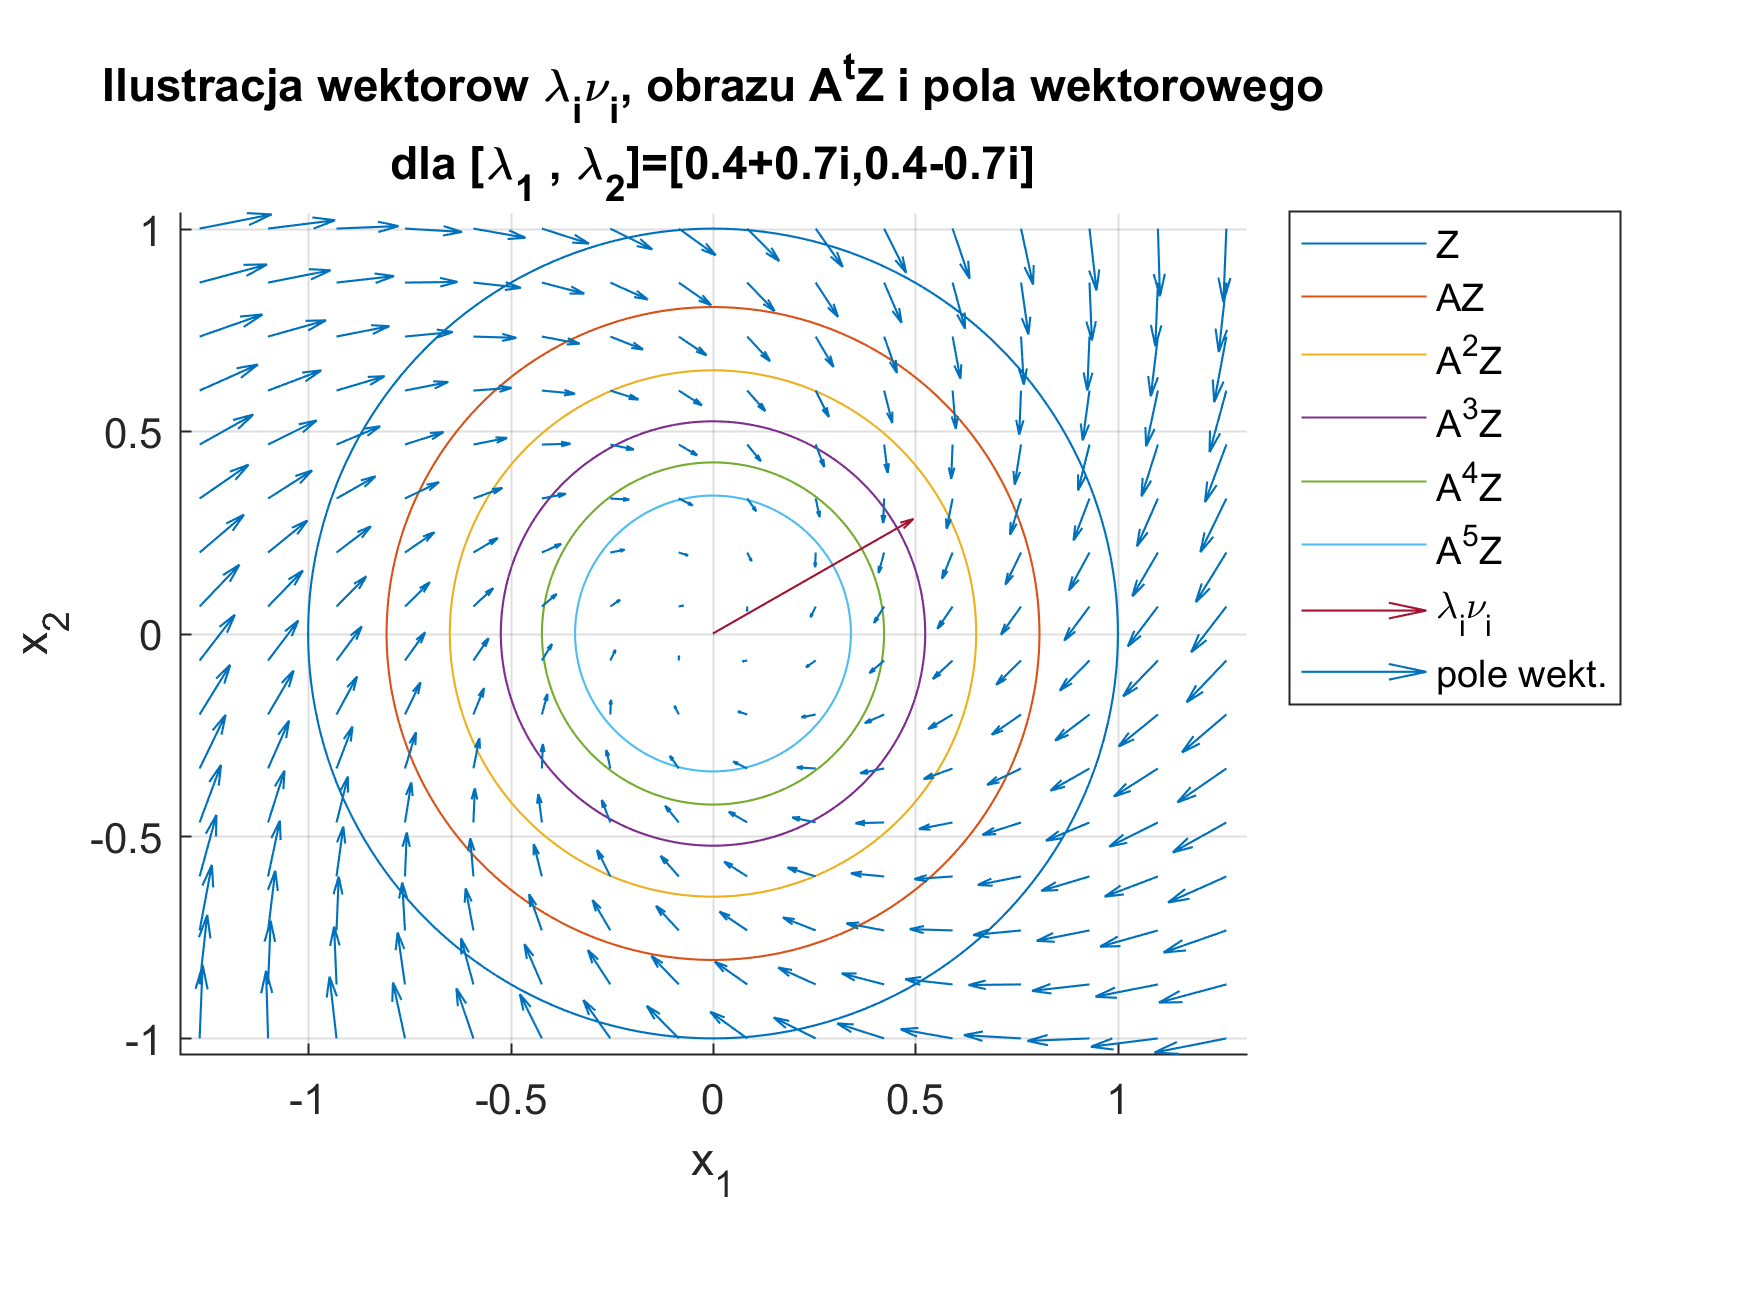
\includegraphics[width=\textwidth]{pole_wektorowe_4+7i_4-7i.png}
    \end{subfigure}
    \caption{Warto\'sci własne $[ \lambda_1, \lambda_2 ]= [ 0.4+0.7i, 0.4-0.7i ]$}
    \label{fig::47ii4-7}
\end{figure}
\begin{figure}[H]
    \centering
    \begin{subfigure}{0.44\textwidth}
        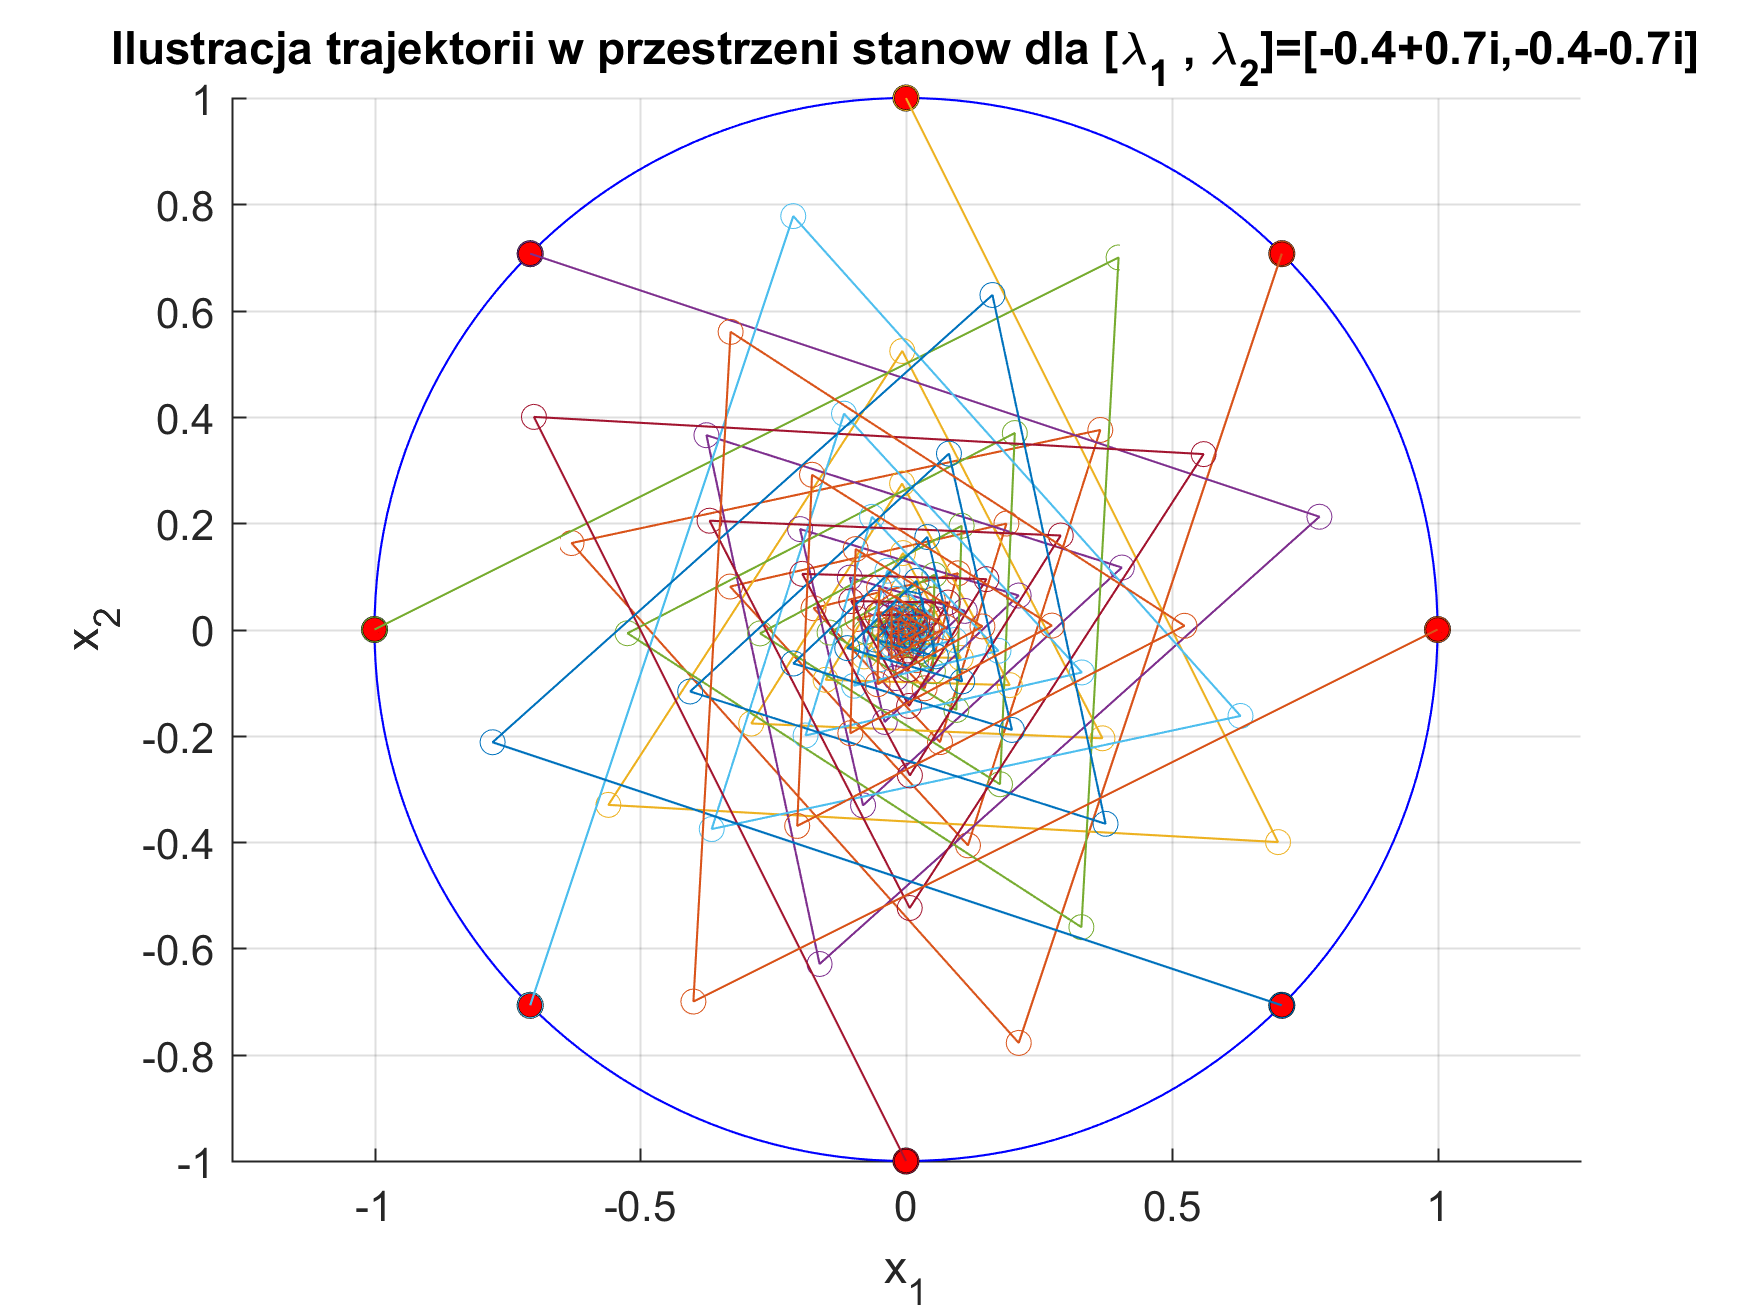
\includegraphics[width=\textwidth]{portret_fazowy_-4+7i_-4-7i.png}
    \end{subfigure}
    \begin{subfigure}{0.48\textwidth}
        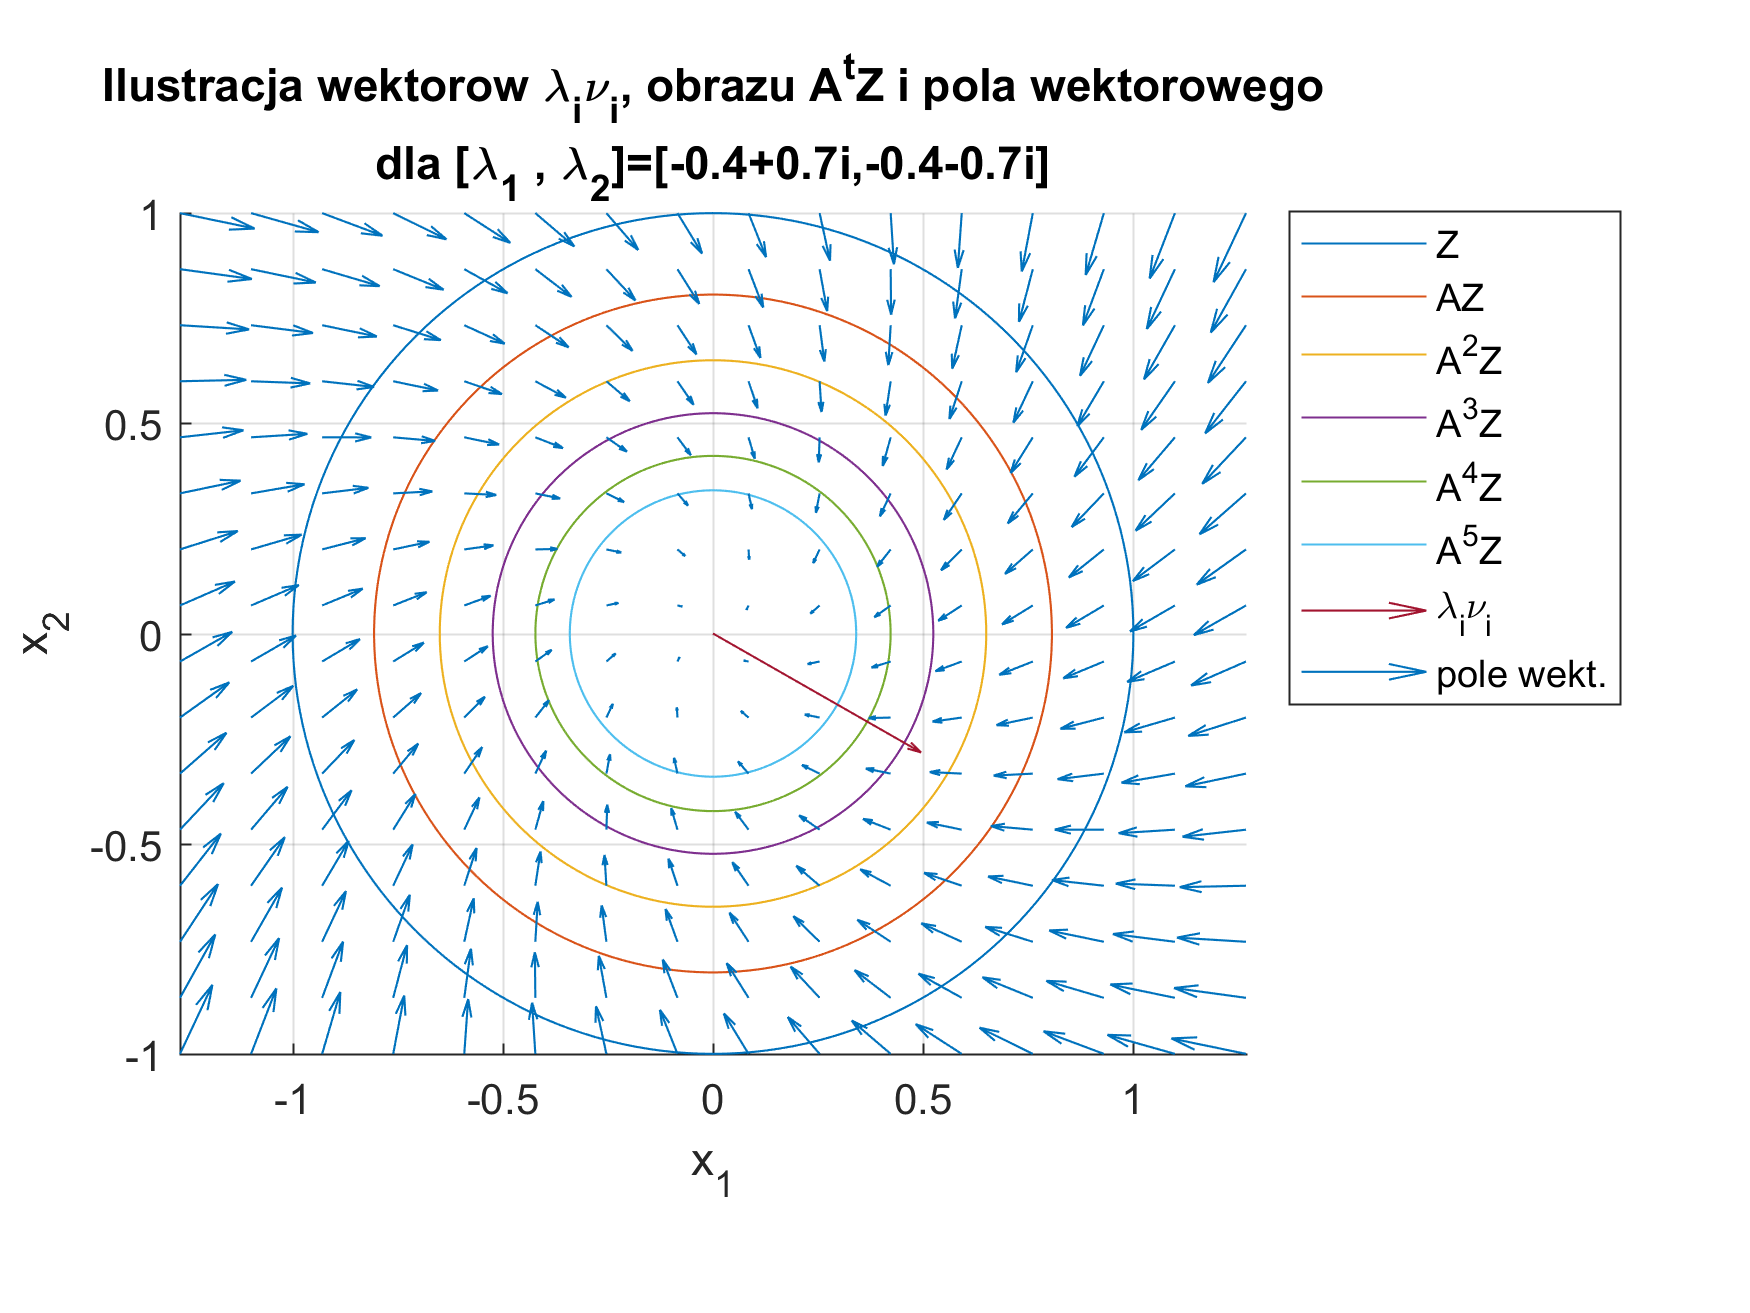
\includegraphics[width=\textwidth]{pole_wektorowe_-4+7i_-4-7i.png}
    \end{subfigure}
    \caption{Warto\'sci własne $[ \lambda_1, \lambda_2 ]= [ -0.4+0.7i, -0.4-0.7i ]$}
    \label{fig::-47ii-4-7}
\end{figure}

 

\section{Wnioski}

Z zamieszcoznych w poprzednim punkcie ilustracji można wyciągnac następujące wnioski:
\begin{itemize}
\item Punkt równowagi układu jest stabilny asymptotycznie (układ jest zbieżny), gdy moduły warto\'sci własnych macierzy \textit{\textbf{A}} są mniejsze od 1 (znajdują się wewnątrz okręgu jednostkowego). Odpowiada to położeniu biegunów transmitancji układów dyskrenych;
\item Układ jest rozbieżny (punkt równowagi układu jest niestabilny), gdy moduł dowolnej warto\'sci własnej macierzy \textit{\textbf{A}} jest większy od 1;
\item Dla warto\'sci własnych będących liczbami zespolonymi sprzężonymi (ze względu na twierdzenie o pierwiastkach wilomianu o współczynnikach zespolonych) występuje charakterystyczna spiralna trajektoria układu, a wektory własne posiadają współrzędne zespolone.
\item W przypadku występowania chociaż jednej warto\'sci własnej o ujemnej czę\'sci rzeczywistej, można zauważyć oscylacje wokół punktu zbieżno\'sci.
\item W przypadku, gdy jedna z wartoci własnych znajduje się na okręgu jednostkowym, za\'s reszta pozostaje wewnątrz okręgu jednostkowego układ jest zbieżny, ale warto\'sć punktu zbieżno\'sci zależy od punktu startowego (ważne jes też również znak czę\'sci rzeczywistej warto\'sci własnej na okręgu - dla dodatnich dochodzimi do punktu zbieżno\'sci, za\'s dla ujemnych osiągamy oscyclacje między doma punktami).
\item Podczas, gdy wszytskie warto\'sci własne macierzy \textit{\textbf{A}} znajdują się na okręgu jednostkowym występują oscylacje między punktami(dla warto\'sci ujemnych cze\'sci rzeczywsitych), bądź pozostanie w punkcie początkowym.
\item Zbieżno\'sć jest zależna od widma macierzy \textit{\textbf{A}}, a odalenie warto\'sci własnej od \'srodka okregu jednostkowego decyduje o szybko\'sci zbiegania(ro\'snie wraz ze zbliżaniem się do \'srodka). Dla warto\'sci własnych \textit{\textbf{A}} równych 0 macierz A jest nilpotentna i układ z czasem dyskretnym zbiega do zera w skonczońej liczbie kroków (z tw. Cayleya-Hamiltona). Dla równych warto\'sci własnych zbieżno\'sć w każdym kierunku jest taka sama.
\end{itemize}
Zatem:
\[
\lambda_i = 
\begin{aligned}
\begin{cases}
0, &dla  |\lambda_i| < 1 \\ 
\infty, &dla |\lambda_i| > 1
\end{cases}
\end{aligned}
\]
Wektory własne $\nu_i$ to wektory, które po przemnożeniu przez macierz \textit{\textbf{A}} nie zmieniają swojego kierunku a jedynie zostają przeskalowane przez warto\'sć równą odpowiadającej mu warto\'sci własnej $\lambda_i$ :
\[ \bold{A}\nu_i = \lambda_i \nu_i \]
Zwiększanie bądź zmniejszanie warto\'sci własnych wpływa przy przekształceniu okręgu jednostkowego przez macierz \textit{\textbf{A}} odpowiednio na na rozciąganie bądź zwęźanie elipsy w kierunkach okre\'slonych przez wektory własne związane z tymi warto\'sciami. Je\'sli iloczyn wektora własnego i odpowiadającej mu warto\'sci własnej $\lambda_i\nu_i$  jest wektorem o długo\'sci większej od 1 to układ jest rozbieżny.

\end{document}